% This file is part of the TheCannon project.
% Copyright 2014 the authors.

\documentclass[12pt, preprint]{aastex}
\usepackage{bm, graphicx, subfigure, amsmath, morefloats}
\usepackage{color}
\input{vc}

%\usepackage{natbib}
\bibliographystyle{apj}

% naming macros
\newcommand{\documentname}{\textsl{Article}}
\newcommand{\sectionname}{Section}
\renewcommand{\S}{\sectionname}
\newcommand{\figurenames}{\figurename s}
\newcommand{\tc}{\textsl{The~Cannon}} 
\newcommand{\apogee}{\textsl{APOGEE}} 
\newcommand{\apokasc}{\textsl{APOKASC}} 
\newcommand{\galah}{\textsl{GALAH}}
\newcommand{\segue}{\textsl{SEGUE}}  
\newcommand{\aspcap}{\textsl{ASPCAP}} 
\newcommand{\gaiaeso}{\textsl{Gaia-ESO}} 
\newcommand{\gaia}{\textsl{GAIA}} 
\newcommand{\rave}{\textsl{RAVE}} 
\newcommand{\matisse}{\textsl{MATISSE}} 
\newcommand{\rotwarn}{\texttt{ROTATION WARNING}} 
\newcommand{\sdss}{\textsl{SDSS-III}} 
\newcommand{\lamost}{\textsl{LAMOST}} 
\newcommand{\aspcapstar}{\textsl{aspcapStar}} 
\newcommand{\apstar}{\textsl{apStar}} 

% math and symbol macros
\newcommand{\set}[1]{\bm{#1}}
\newcommand{\starlabel}{\ell}
\newcommand{\starlabelvec}{\set{\starlabel}}
\newcommand{\mean}[1]{\overline{#1}}
\newcommand{\given}{\,|\,}
\newcommand{\teff}{\mbox{$\rm T_{eff}$}}
\newcommand{\kms}{\mbox{$\rm kms^{-1}$}}
\newcommand{\feh}{\mbox{$\rm [Fe/H]$}}
\newcommand{\xfe}{\mbox{$\rm [X/Fe]$}}
\newcommand{\alphafe}{\mbox{$\rm [\alpha/Fe]$}}
\newcommand{\mh}{\mbox{$\rm [M/H]$}}
\newcommand{\logg}{\mbox{$\rm \log g$}}
\newcommand{\noise}{\sigma_{n\lambda}}
\newcommand{\scatter}{s_{\lambda}}
\newcommand{\pix}{\mathrm{pix}}
\newcommand{\rfn}{\mathrm{ref}}

\begin{document}

\title{\tc:\\ A data-driven model for stellar parameter determination}
\author{M.~Ness\altaffilmark{1},  
David~W.~Hogg\altaffilmark{1,2,3}, 
H.-W.~Rix\altaffilmark{1}, 
A.~Ho\altaffilmark{1}, 
G.~Zasowski\altaffilmark{4,5}}
\altaffiltext{1}{Max-Planck-Institut f\"ur Astronomie, K\"onigstuhl 17, D-69117 Heidelberg, Germany}
\altaffiltext{2}{Center for Cosmology and Particle Physics, Department of Phyics,
             New York University, 4 Washington Pl., room 424, New York, NY, 10003, USA}
\altaffiltext{3}{Center for Data Science, New York University, 726 Broadway, 7th Floor, New York, NY 10003, USA}
\altaffiltext{4}{NSF Astronomy and Astrophysics Postdoctoral Fellow}
\altaffiltext{5}{Department of Physics \& Astronomy, Johns Hopkins University, Baltimore, MD, 21218, USA}
\email{ness@mpia.de}

\begin{abstract}%
New spectroscopic surveys offer the promise of consistent stellar
parameters and abundances (`stellar labels') for hundreds of thousands
of stars in the Milky Way. 
These labels are usually derived by comparisons with physics-based
model spectra, which are technically challenging, and often use only a
modest fraction of the spectral pixels. 
In many cases, however, there is a sub-set of \emph{reference}
objects for which the stellar labels are known with high(er)
fidelity; this is the case for \tc.
From the reference stars, \tc\ learns by fitting a very flexible
model how the flux in each pixel of a continuum-normalized spectrum
depends on the `known' stellar labels; \tc\ then exploits this same
dependence to derive new labels for the non-reference stars.
We illustrate \tc\ by applying it to the spectra of 55,000 stars from
\apogee\ DR10. 
We take \teff, \logg\ and \feh\ as the labels, and 543 stars in 19
clusters as the reference objects. 
\tc\ is very accurate; its stellar labels compare well to the 37,500
stars for which \apogee\ pipeline (\aspcap) labels are provided; we
obtain rms differences of $\delta\teff< 100$~K, $\delta\logg< 0.2$~dex
and $\delta\feh< 0.1$~dex.
Aside from the modeling of the training-set stars (which could happen
in another dataset or at another wavelength), \tc\ makes no use of
stellar models nor any linelist; its biggest limitation is that it
requires a training set that spans the label-space. 
The method degrades very weakly with signal-to-noise; \tc\ delivers
the labels with good fidelity even at one ninth the
\apogee\ observing time. 
We discuss the limitations of \tc, and point out the potential of this
approach to bring different spectroscopic surveys onto a consistent
scale of stellar labels if they have sufficient objects in common.
\end{abstract}

\keywords{%
methods: data analysis
---
methods: statistical
---
stars: abundances
---
stars: fundamental parameters
---
surveys
---
techniques: spectroscopic
}

\section{Introduction}\label{sec:Intro}

The vast spectroscopic stellar surveys of recent years (e.g., \segue\ \citep{Beers2006}, \rave\ \citep{Steinmetz2006}, \lamost\ \citep{Newberg2012}, \apogee\ \citep{Majewski2012}, \gaiaeso\ \citep{Gilmore2012}, \galah\ \citep{Freeman2012}) hold tremendous astrophysical promise, but at the same time present formidable data analysis and modeling challenges. 
One of these challenges lies in consistently and accurately determining what we call ``stellar labels'', that is, stellar parameters and element abundances, from survey spectra. 
These labels are usually determined from comparison of the data with synthetic model spectra, with approaches often 
customised specifically to the particular wavelength region of a given survey \citep[e.g.,][]{ Lee2006, Boeche2011, Liu2014, Meszaros2013, Sm2014}. 

The stellar photosphere models that are relied upon for stellar label determination have physical ingredients that are incomplete and simplified. 
For computational feasibility, almost always 1D stellar photosphere models are adopted for large surveys, often assumed to be in local thermal equilibrium; these approximations are both severe. 
In many cases, the model spectra do not account for all relevant  molecular opacities, for convection, stellar winds, and the chromosphere. 
As a consequence, it happens that different research groups obtain discrepant results for same stars, resulting from analysis across different wavelength regions and different input assumptions and methods used \citep[e.g.,][]{Hinkel2014, Jofre2014, AP1999}. Even when the input assumptions are held fixed, differences in the employed analysis methods lead to substantial differences in assigned labels \citep[e.g.][]{Sm2014}.

Stellar labels are commonly determined by fitting a grid of model spectra (with known labels) to the data using some minimisation technique, often restricted to a masked portion of the spectrum that is focussed on the absorption line (regions) deemed to be most reliable or relevant. 
Stated minimal signal-to-noise requirement to obtain robust labels in this way are $SNR\sim 100$ per resolution element, especially if the labels are to include individual element abundances. 
Often, a post-calibration procedure is applied to bring the stellar labels derived by such a fitting pipeline in accord with external information of higher fidelity: for example with stellar labels from benchmark stars studied at high resolution or well characterised open and globular cluster stars \citep[e.g.,][]{Meszaros2013, Freeman2013}
In practice, different surveys or different pipelines end up delivering labels with different calibrations:
Either their stellar parameter or their abundances are on slightly different scales; this complicates
inter-survey comparisons and constitutes major challenge of the era of such large datasets. 

In this paper we propose and lay out a data-driven approach to deriving stellar labels from stellar spectra in the context of large spectroscopic surveys,
which we dub ``\tc''\footnote{The name \tc\ is inspired by the astronomer Annie Jump Cannon,
who was the pioneer in producing stellar classifications without any input of physical models!}.
The main practical strengths of \tc\ are that it requires no physical model of the spectra, it is enormously fast, it can obtain labels of comparable accuracy to that quoted in current physics-based approaches
 but at far lower signal-to-noise ratio, and it offers a consistent way to cross-calibrate surveys. 
To achieve this, \tc\ relies on the existence of a subset of objects within a survey
(\textit{reference objects}), for which the stellar labels are known sufficiently well and cover label space sufficiently.

In this context, the term ``\emph{labels}'' refers to the pieces of information
that characterize and determine a stellar spectrum; these labels are commonly and sensibly split into \emph{stellar parameters} and \emph{element abundances}, although in the context of \tc\ it makes sense to treat them on a par. 
In most cases, it suffices to think of the labels as \teff , \logg, and the element abundances \xfe, athough stellar rotation, microturbulence, age, and so forth can also be thought of as labels.
It is central to the approach we lay out here that stars with the same labels have (nearly) identical spectra and that spectra vary smoothly with label changes. 
This must be true, if the set of labels is comprehensive enough so that it fully specifies the star; but if the labels are (for example) only \teff, \logg\ and \feh\ then this is an approximation.

There are fundamentally two steps in \tc. 
The first step, or \textit{training step} in \tc\ is to create from the spectra of the \textit{reference objects} a very flexible generative model (with $\sim 80,000$ parameters) that describes a probability density function (pdf) for
 the flux at every pixel in the continuum-normalized spectrum as a function of stellar labels.
The second step, or \textit{test step}, assumes that this same generative model holds for all the other objects in the survey (dubbed \textit{survey objects}). 
Then, the spectra of the \textit{survey objects} and the generative model from the \textit{reference objects}
allow us to solve for---or infer---the labels of the \textit{survey objects}. 
Taken together the \textit{training step} and the \textit{test step} effect a \textit{label transfer},
transfering the known labels in the reference objects to the survey objects.

To make such an approach straightforward, we must assume that the \textit{reference objects} and the \textit{survey objects} were observed with the identical instrumental set-up, a condition well satisfied with the large surveys listed above. 
We take the generative model for the continuum normalized flux at each of $N_\pix$ pixels to be a polynomial function of all the labels, and hence the model is defined by its $N_\pix$ sets of polynomial coefficients. In practice, there may be different circumstances that make stars suitable reference objects. 
They may be members of star clusters: there, external data and the fact that clusters are in good approximation single stellar populations (which have to fall onto an isochrone) lend credibility to their stellar labels. 
Alternatively, reference objects could be stars for which labels have been derived separately from spectra of particularly high signal to noise, or at other ``easier'' or more extensive wavelength regimes (for example, in the optical as opposed to the infrared). 
Finally, they may be subsets of stars for which other approaches to get stellar parameters (for example, astroseismology) may provide accurate stellar parameters.

With this two-step procedure of training on spectra of reference objects and then transferring the label information to the survey objects, \tc\ falls into the class of \emph{supervised methods} in machine learning. 
However, what we implement is very different in a crucial way from standard supervised methods for regression, such as support vector machines, random forests, and deep learning.
These other methods also try to fit a very flexible model to the training data at training time
and deploy that model on the test data at test time.
The important difference, however, is that \tc\ is a \emph{generative model} of the observed spectra:
That is, it constructs, as a function of labels, a probability density function (pdf) for the observed
flux as a function of wavelength. 
This makes \tc\ a bespoke method, not cleanly falling into any established machine-learning methodology.
However, it gives us the enormous advantage that we can account for the uncertainties in the spectral data,
including all the issues of heteroscedasticity and missing data.
It also makes the method agnostic about signal-to-noise.
This point is technical, but important:
In many real cases the training data will be much higher in signal-to-noise than the test data
(standard stars tend to be bright and well observed).
A method that does not properly account for the observational uncertainties will not transfer labels from high signal-to-noise reference objects to lower signal-to-noise survey objects with high fidelity.
In what follows, we show that \tc\ behaves very well as the signal-to-noise (or observing time) is decreased.

In this paper we use \apogee\ as the sole example. 
However, \tc\ can be applied to any stellar survey.  

Our most basic implementation of \tc\ that we present includes only three labels, but this can easily be extended to additional labels  (for example, \alphafe, \xfe) and also more comprehensive models (for example, Gaussian processes). 
Additionally, as we are using the information in every pixel, this methodology is effective at determining labels at lower signal to noise (SNR) than minimisation techniques.

\tc\ is similar to the MATrix Inversion for Spectral SythEsis (\matisse) procedure
for derivation of stellar parameters \citep{RB2006} in that it uses the full spectrum
(and not just a line list) for label determination.
However, \matisse\ employs a large grid of synthetic spectra
and is thus limited in all the ways that physics-based methods are limited.
That said, a big part of why \tc\ is successful at lower signal-to-noise
is that it uses all of the pixels in the data.

We have adopted a bottom-up approach for \tc, starting with the most basic implementation and successively adding complexity to the generative model to determine the least complex implementation which works.  
In laying out the methodology of this approach we firstly describe the \apogee\ dataset and the way we process the data for both reference objects (543 stars) and survey objects ($\sim$ 55,000 stars from DR10). 
We then describe perhaps the simplest implementation of label-transfer possible, using a first-order linear model. We found this first-order model to be insufficiently flexible to describe the labels of the stars and so we extended our model to quadratic form, which satisfactorily describes the label-space of the training data.
The success of this model is demonstrated by running \tc\ through the DR10 data available through the SDSS-3 data server, the results for which we provide in an online machine-readable table. % for about 42,000 DR10 stars. 

\section{Data}\label{sec:Data}
\tc\ expects (in its simplest form, presented here)
all spectra---for reference and survey objects---to be continuum normalized in a consistent way,
and sampled on a consistent rest-frame wavelength grid, with the same line-spread function.
It also assumes that the flux variance, from photon noise and other sources, is known at each specral pixel of each spectrum.
In principle, \tc\ , as described below, is applicable to any large, homogeneous spectroscopic data set
meeting these criteria.
Here, we use the \apogee\ data \citep{Ahn2014} to illustrate and showcase \tc.
Because all of the exposition of the method underlying \tc\ involves specificities of the data,
we spell out the characteristics of the \apogee\ data and our adjustments to it in +\sectionname~\ref{sec:Apogee_as_worked_Example}.

\subsection{Choosing reference objects for the training step}
\label{sec:ReferenceObjects}

For the training step in \tc\ we must choose a set of reference (or training) objects for which we have spectra from the survey under consideration and \emph{also} high-fidelity labels (that is, stellar parameters and element abundances that are deemed both accurate and precise).
The set of reference objects is critical, as the label transfer to the survey objects can only be as good as the quality of the reference label set. 
Also, as \tc\ may have to interpolate and extrapolate to new parts of label space as
it encounters new kinds of spectra among the survey objects, the quality
of the label transfer depends on the extent to which the reference objects
cover label space and the density with which they cover it.
The performance of a data-driven model like \tc\ will depend strongly on the size and quality of its training set of reference objects, much more strongly than the square-root of the number!

In practice, also for the \apogee\ data,
a good set of reference objects can be built from 
members of well studied open and globular clusters that have been observed in the context of the survey.
There is a variety of reasons why the stellar labels for cluster stars may be particularly accurate and robust.
For one, they could have their labels derived from independent, high resolution spectral analysis of these
stars, e.g. from observations in a well understood portion of the optical wavelength region. The
labels for the reference objects only have to be accurate and trustworthy; but they are of course a property of the
star, and hence do not have to arise from the survey data at hand. They may have been derived from different data.

For the case of \apogee, we will use as reference objects 543 members of 19 globular and open clusters data observed for the
calibration of their abundance pipeline \citep{Meszaros2013}. In their stellar labels they span the range of $3500<\teff<5300$~K, $0<\logg<5$ and $-2.5<\feh<0.45$. 
Exactly which stellar labels we adopt for these reference objects is critical to the subsequent output, and hence 
we discuss it in detail in \sectionname~\ref{sec:ApogeeRefLabels} .

% MKN:  SHOULD THIS BE IN THE MAIN TEXT?  note there are 20 in their list but 1 gc has only 1 star and the abundance looks incorrect to me. DWH: No I don't think we should call this out explicitly in the paper it's more pointing out what I think is an error than adding anything useful. 
Another reason why cluster members make for good reference objects is because we can expect their stellar parameters to fall onto a single isochrone and to have near-identical abundances (at least for open clusters). This provides additional constraints on the labels.
We exploit that expectation in the case of \apogee\ and define ``Isochrone-corrected labels'', where we use Padova isochrones at the literature age and \feh\ of each cluster (cf. Figs. \ref{fig:trainingaspcap} \& \ref{fig:trainingisochrone}, and \sectionname~\ref{sec:ApogeeRefLabels}).

A spectral survey may also contain other sub-sets of objects with labels of particularly high fidelity that can serve as reference objects, such as the stars with \logg\ from Kepler's astroseismology in \apogee . Or, one could simply choose as reference objects the subset of stars in a survey with the highest signal-to-noise spectra, if one can reasonably assume that the labels derived for those objects from physics-based spectral modelling are accurate. So, there are various sensible ways to choose the set of reference objects.

%run -i fitiso_apogeetempfeh_paperrework2.py
%makeonisochrone_training_4panel_revb.py
\begin{figure}[h!]
\centering
    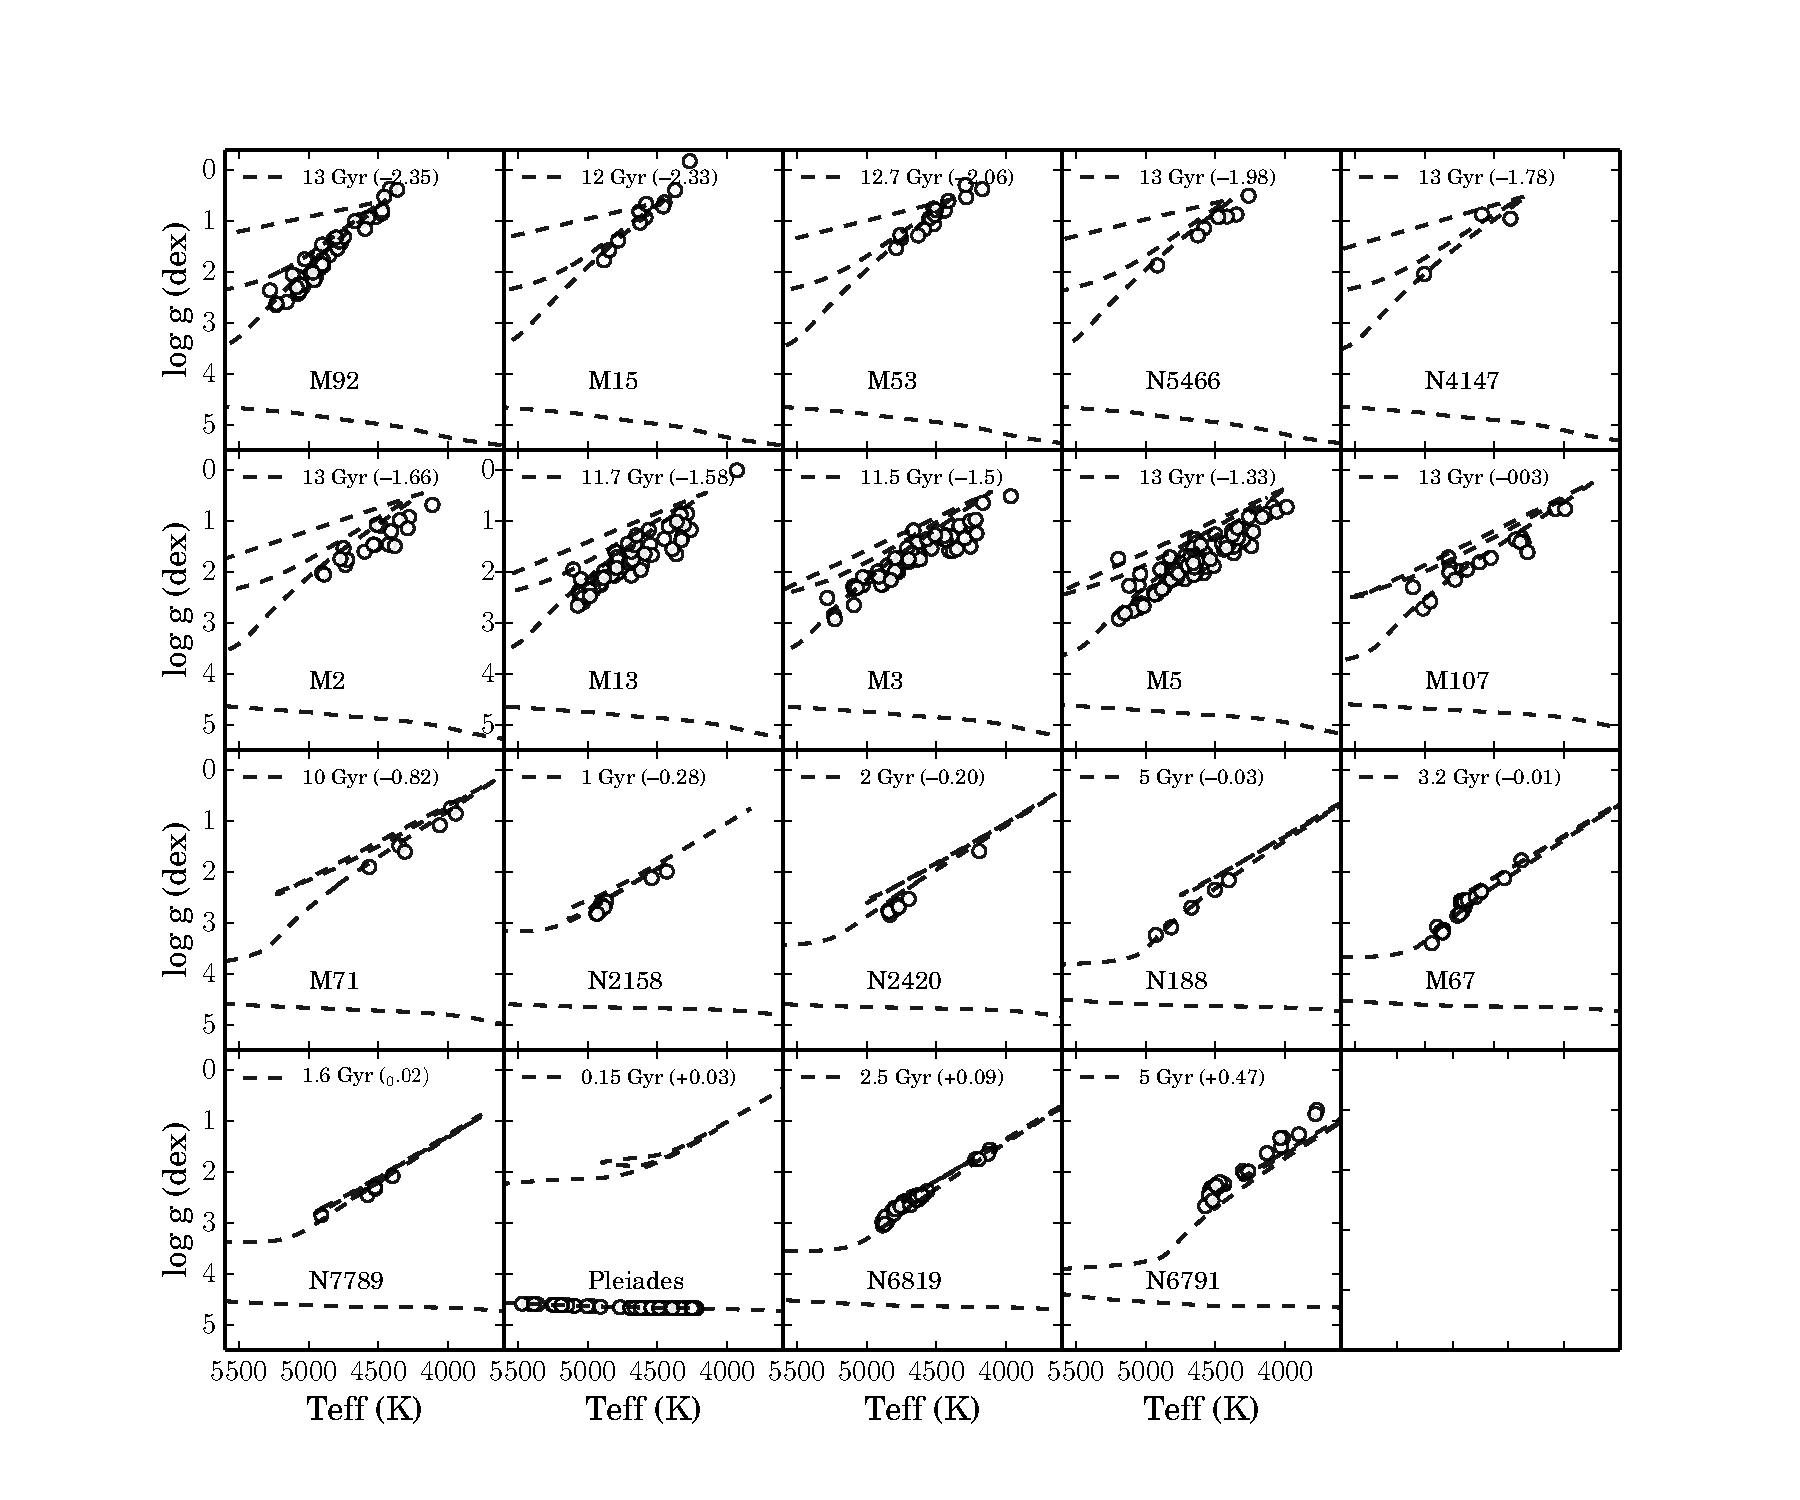
\includegraphics[scale=0.33]{./plots/training_aspcap.pdf}
\caption{\aspcap-corrected DR10 labels  for the training step in \teff-\logg\ plane for 543 stars in the 19 clusters for which parameters are provided by APOGEE \citep{Meszaros2013}. The age and \feh\ of the isochrones (in parentheses) is shown in each sub-panel. All labels adopted from the \aspcap\ corrected values of DR10 except for the Pleiades. }
\label{fig:trainingaspcap}
\end{figure}

\begin{figure}[h!]
\centering
  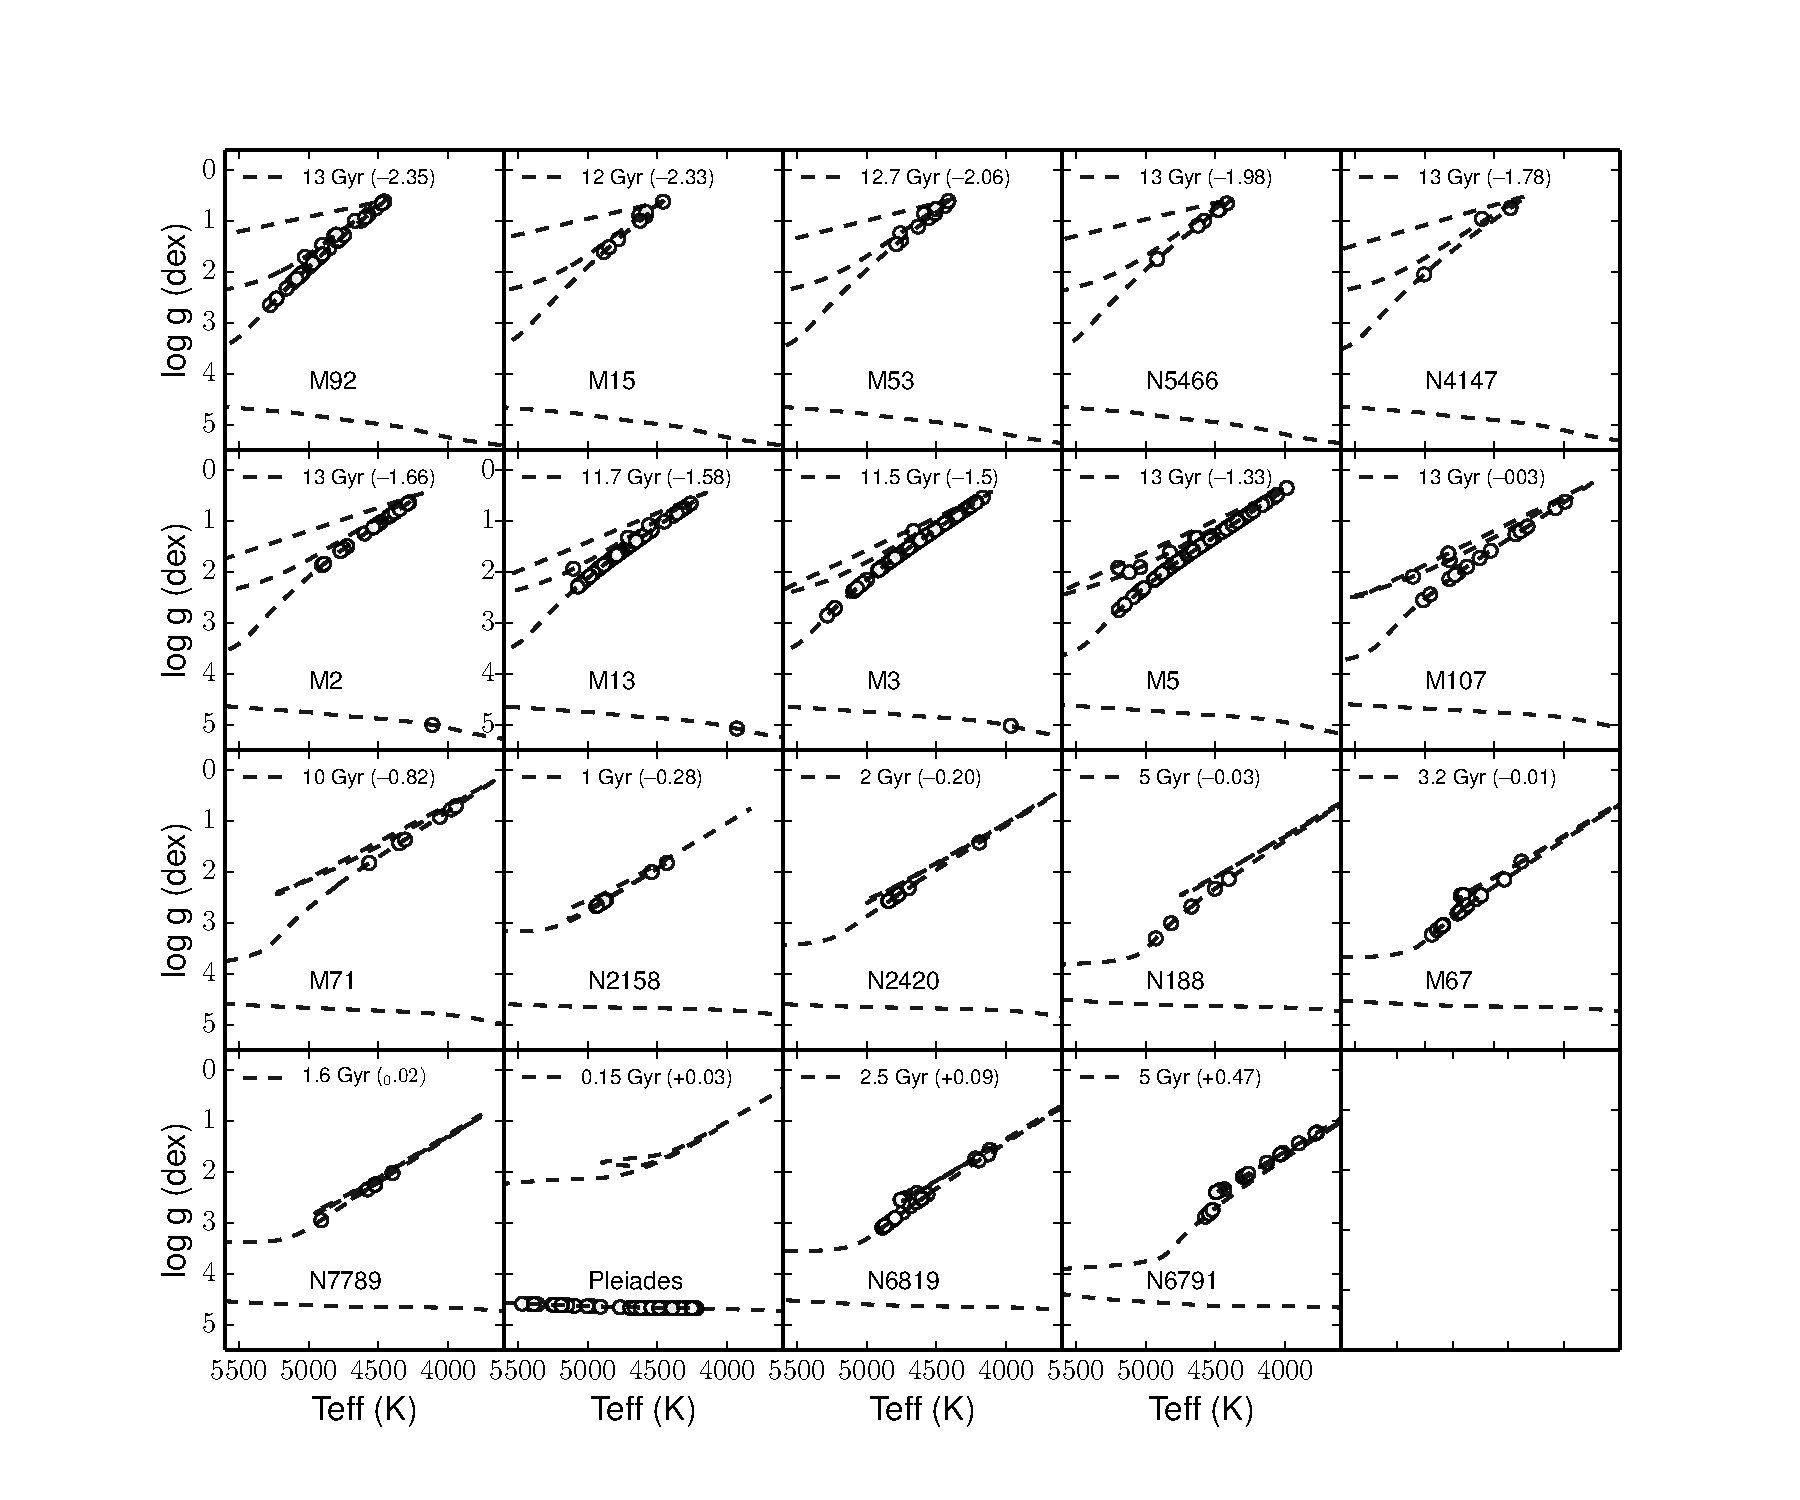
\includegraphics[scale=0.33]{./plots/training_mkn2.pdf}
\caption{Stellar labels for all reference objects as is \figurename~\ref{fig:trainingaspcap}, except that the \logg\ values have been adjusted from the \aspcap-corrected value to exactly match the isochrone, we refer to this set of labels as  ``isochrone-corrected'' labels to differentiate them from the correction in \figurename~\ref{fig:trainingaspcap}.  }
\label{fig:trainingisochrone}
\end{figure}

\subsection{Consistent Continuum Normalization}\label{sec:ContNorm}

\tc, as we present it here, operates on continuum-normalized spectra.
Continuum-normalization that is based on quantiles of the data (medians or 90-th percentiles or the like)
are very signal-to-noise dependent, e.g. because pixels that are clearly \emph{not} continuum in high signal-to-noise
spectra are completely consistent with being continuum at lower signal-to-noise.
Therefore, to make \tc\ as independent of signal-to-noise (hereafter ``SNR'') as possible,
we base the continuum estimation on a pre-tabulated set of wavelength locations that we know
(iteratively, from running \tc\ itself) are not strongly affected by absorption lines.

To initialize the continuum-pixel determination,
we define a preliminary pseudo-continuum normalisation by 
using polynomial fit to an upper quantile (for example, 80 or 90~percent) of the spectra
 in the \apogee\ pipeline \citep{Meszaros2013}, determined, for example, from a running median.
  This is effective, but SNR dependent.
  
After a training step with spectra of reference objects that have been  normalized  by this pseudo-continuum,
the \tc\ can provide an improved identification of continuum regions in the spectrum: 
we take those pixels to be continuum that show nearly unity flux in the spectral model's baseline spectrum (see \sectionname~\ref{sec:spectralmodel}), and at the same time show almost no dependence in their normalized flux on the stellar labels.
That is, we can determine with the \tc\ the `true' continuum, using the model derived from the pseudo-continuum normalised spectra for the reference objects provided by \apogee, as described in \sectionname~\ref{sec:results}. This constitutes a data-driven method for finding continuum pixels, and we find it to have only a very small systematic dependence of the spectra on SNR (see \sectionname~\ref{sec:ApogeeContinuum}).

We are now in a position to determine the continuum by least-squares fitting a low-order Chebyshev polynomial, but only to these just determined continuum pixels.
For \apogee\ we treat each of the three chips separately, and find a 2nd-order Chebyshev polynomial to be sufficient to apply to the pseudo-continuum normalised data provided by \apogee\ . We apply this normalisation to both \aspcapstar\ and \apstar\ files. Treating the three chips separately, we fit the polynomials over the wavelength regions of (i) 15150-15800 $\AA$, (ii) 15890 - 16430 $\AA$ and (iii) 16490 - 16950 $\AA$. Fitting a polynomial has the disadvantage that they are poorly constrained at the edges of the data. An alternative implementation could use a more sophisticated sine or cosine function in place of a polynomial fit. 


\figurename~\ref{fig:norm} shows an example of this normalisation applied to survey spectra with different labels.
To illustrate the result, \figurename\ shows typical \apogee\ spectra and demonstrates how the spectra 
vary as a function of metallicity at a given temperature , and as a function of temperature at a given metallicity. 
For a clearer view of individual absorption line features, we use narrower regions marked in this \figurename, (A) and (B), for all subsequent examination of the spectral data. 


%. The continuum pixels used for the Chebyshev polynomial fit are shown in the black points.

%made with makecontin_data2.py
\begin{figure}[h!]
  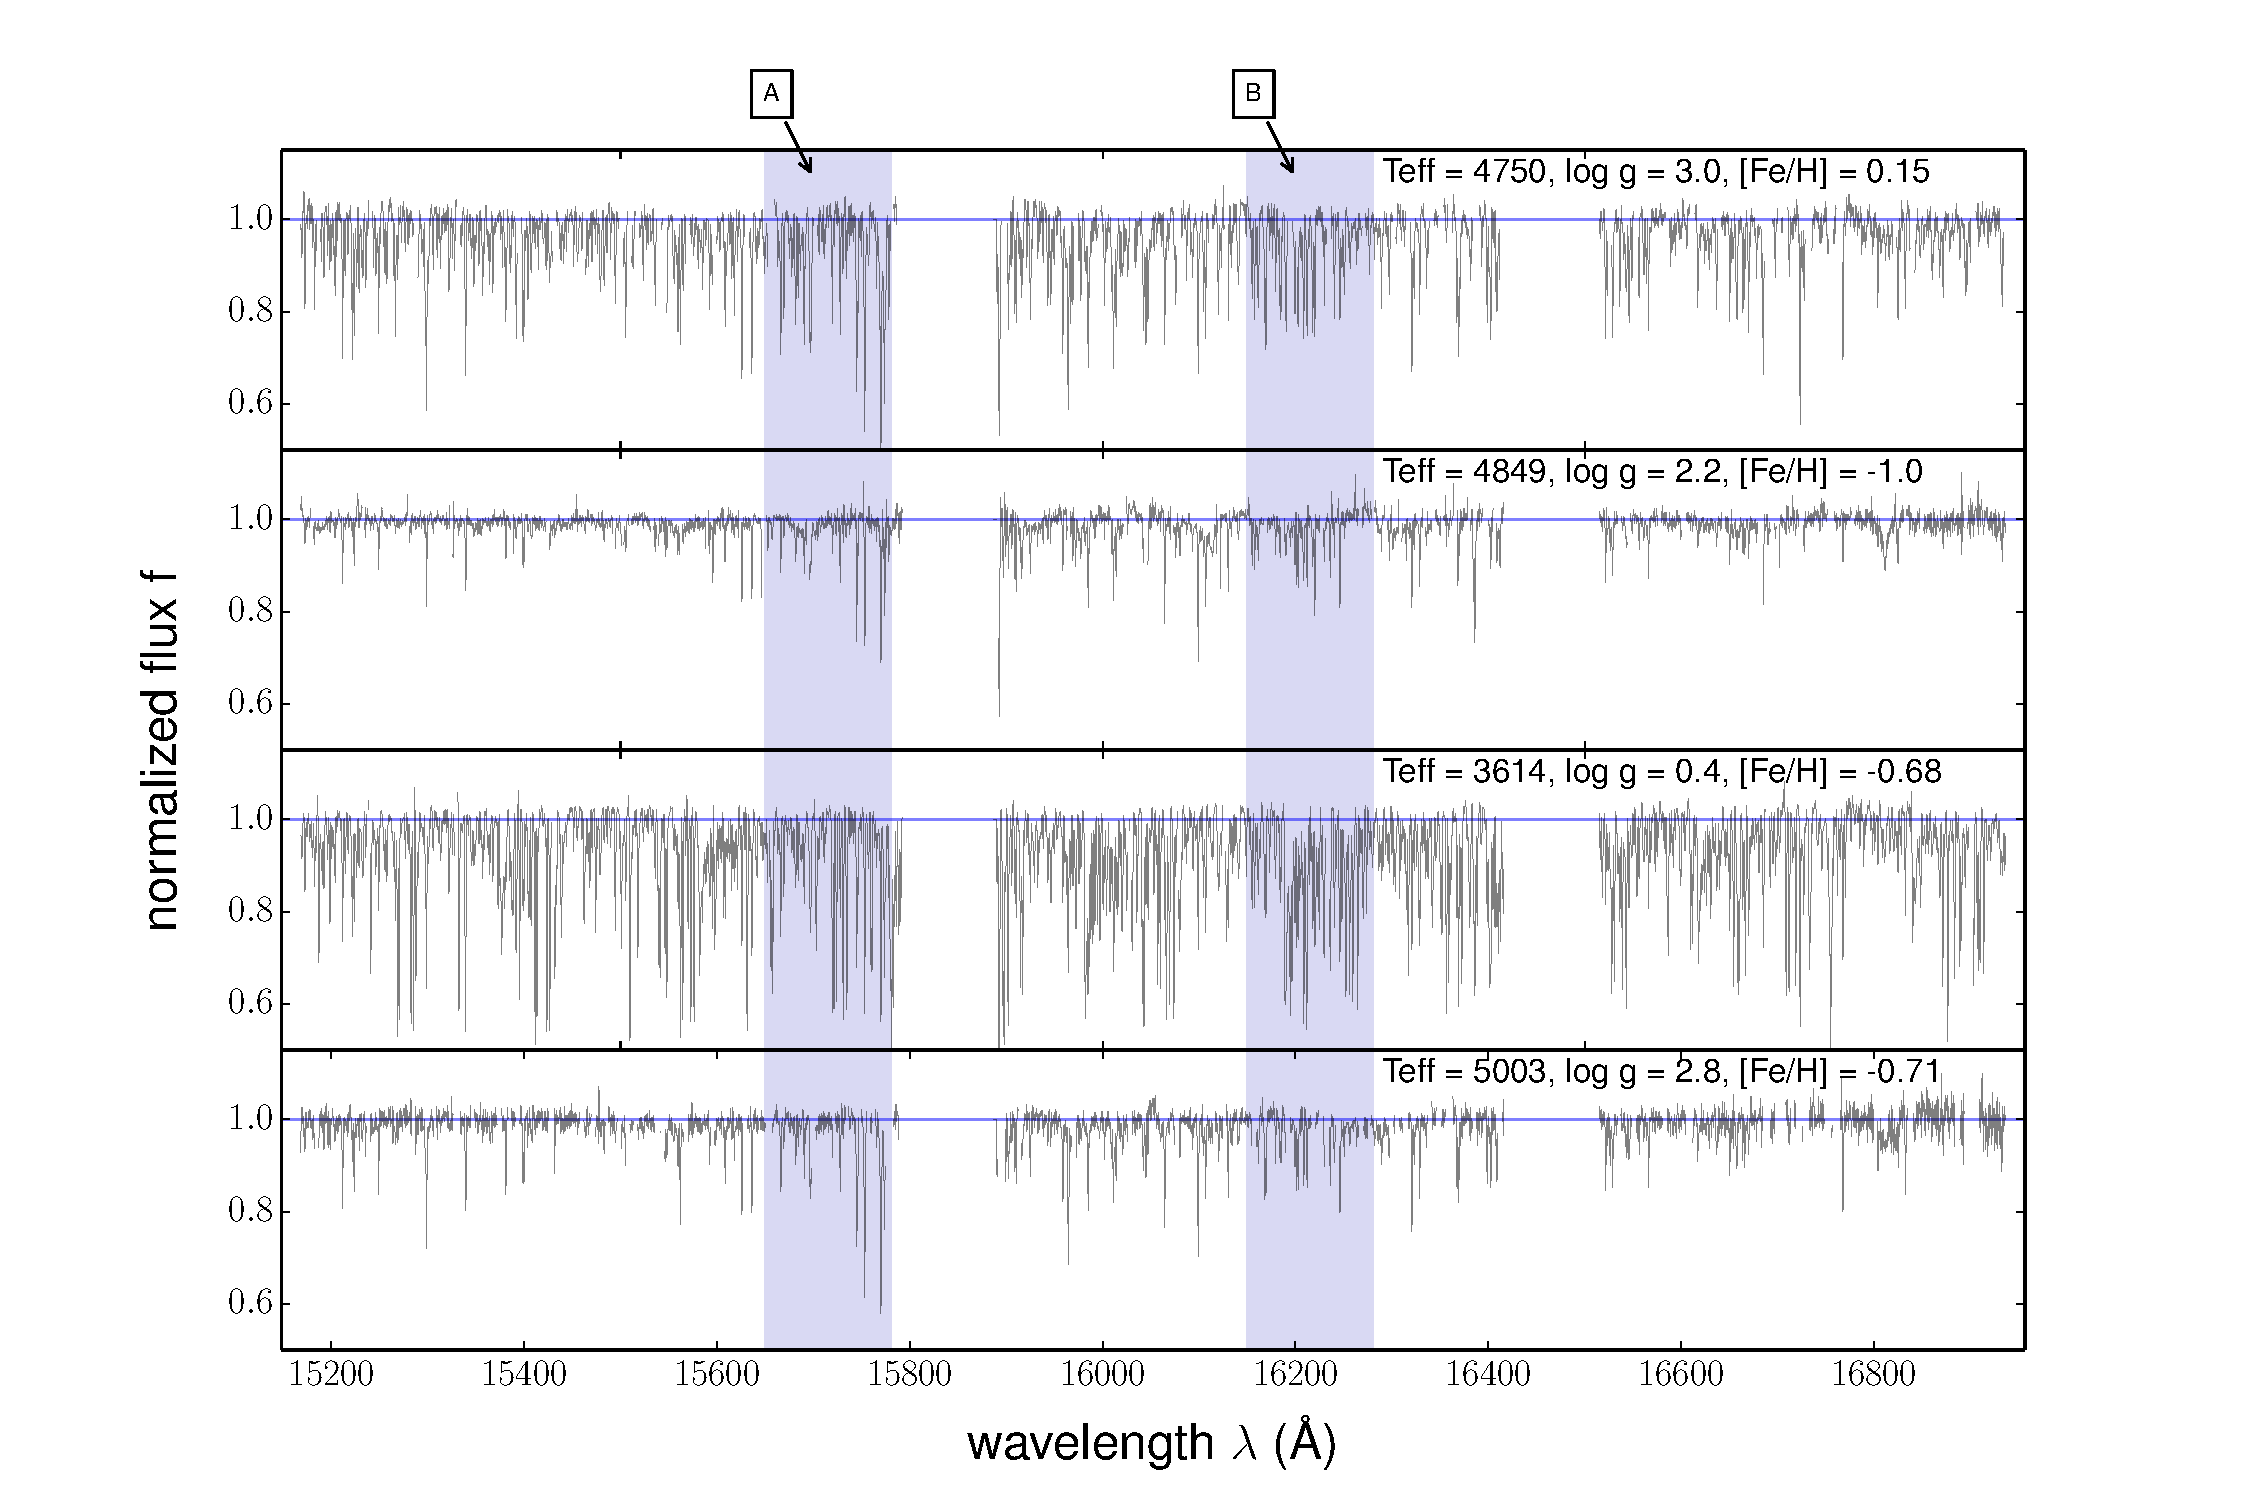
\includegraphics[width=\hsize]{./plots/four_examples3.pdf}
\caption{Continuum normalised spectra for stars across a range of stellar labels; at top, two stars of similar temperatures at different metallicities and at bottom, two stars of similar metallicities and different temperatures. The grey shaded regions A and B indicate \apogee\ sample wavelength regions used for subsequent \figurenames\ in the paper.}
\label{fig:norm}
\end{figure}

\subsection{Specifics of the APOGEE Data Set}
\label{sec:Apogee_as_worked_Example}

In the application of \tc\ to  \apogee, we start with the \aspcapstar\ and \textit{apstar} files of DR10,
which are reduced and resampled. 
The \textit{apstar}  data are not pseudo-continuum normalised by \apogee\,
which will enable us to evaluate the performance of \tc\ at lower SNR, by testing using the individual visit spectra provided in these files. 

The pixel-by-pixel inverse variances are critical for all steps of the \tc\ : continuum normalization, training step and test step.
Aside from photon noise, a number of other factors can contribute to the errors of any pixel in \apogee\ specta: poor sky subtraction, cosmic rays, reduction induced errors, high persistence and other noise sources. In addition to the variance arrays, one must also use any bad pixel masks, where the
inverse variance and weighing of that pixel becomes $\sim$ 0. 

The resampled, reduced and combined spectra are available for 49,200 stars in 150 of the 170 DR10 fields in the \aspcapstar\ files. There are a further 4800 stars in 20 fields taken in commissioning only in DR10 which are available in the radial velocity combined but not continuum normalised data format in the \apstar\ files and a further 3100 stars taken during commissioning across different fields. 
The commissioning data, for which the \aspcap-corrected labels are not all provided in the DR10 release, is only available in the radial velocity combined but not continuum normalised data format in the \apstar\ files. 
We use the \apogee -provided bad pixel masks for the \textit{apStar} files run through \tc .

We did attempt to apply the \tc\ to the commissioning data, but could not evaluate the fidelity of these results as the line spread function of the commissioning data are different from the main survey and consequently the reference dataset of stars in the training step. 
Therefore, although we similarly process the \apstar\ spectra, returning the labels for these stars in our online table of DR10 parameters, the reliability of these is uncertain and they are subsequently flagged as commissioning data (see Table 1).


\subsubsection{Labels for the Reference Objects in APOGEE}
\label{sec:ApogeeRefLabels}

Which labels to adopt for the reference objects used in \tc 's training step is a critical issue
in any survey. We discuss two options here for \apogee . 
First, we adopt the DR10 ``\aspcap\ corrected'' stellar parameters that are available for each of the reference objects as their labels, in order to place the output of \tc 's test step for the survey objects on the \apogee\ \aspcap\ scale (\figurename~\ref{fig:trainingaspcap}). ``\aspcap\ corrected'' labels were not available for the cluster comprised of main sequence stars, the Pleaides cluster and for this cluster we made our own corrections in \teff\ and \logg\ and assumed a single literature value for the \feh\ label, as described below. 
The reference set of stars we use is the very same stars used by \apogee\ to post-calibrate the output of \aspcap\ to a physical stellar parameter scale \citep{Meszaros2013}.
Adopting the \aspcap\ corrected labels provided and documented by \apogee\ has the important advantage 
that we can test exactly how well we can reproduce the results from \apogee\ for the survey stars via label-transfer from only 543 stars.

The corrections to the labels made by \apogee\ based on the cluster data are applied to the immediate output of the \aspcap\ pipeline that arose from comparisons to a library of stellar models.
Temperature corrections are determined by comparing the infrared flux temperatures of the stars \citep{gonzalez2009}, \logg\ corrections are from the offset between \aspcap\ results and Kepler results for common stars and \feh\ corrections are from the difference between the \aspcap\ and  the literature value of each cluster.  
The \apogee\ corrections determined in \citet{Meszaros2013} are valid only for stars with \logg\ $<$ 3.5 and are not implemented for the dwarfs.  We adopt the \aspcap\ corrected \mh\ values for these clusters and these are corrected to the \feh\ of the clusters and so we adopt this label as an \feh\ (that is, this label from \apogee\ therefore, does not explicitly use \feh\ lines, but is derived from an \feh\ correction). 
The analysis in \citet{Meszaros2013} is restricted not only to giants but also stars with SNR $>$ 70, determined to be the minimum SNR for reliable stellar parameters by \apogee.

These corrections implemented by \apogee\ in \teff, \logg\ and  \feh\ place the giants in the cluster stars on or near the iscohrones (see \figurenames~7 and 8 in Meszaros et al., (2013)).  
As there are no \aspcap\ corrections implemented for the 64 main sequence stars among the reference objects that we use, 
we instead determine temperatures for these dwarfs, which are all in the Pleiades, directly using same correction method 
as in \citet{Meszaros2013}. 
We determine the infrared flux temperature for the stars from \citet{gonzalez2009} and apply a correction to 
the \aspcap\ output based on the offset in the temperature scales. For the dwarf stars in the Pleiades, we find the following relation:
 $T_{\mbox{corrected}}$= 0.855*T$_{\mbox{\textit{\aspcap}}}$ + 1206.7.

We do not attempt an individual metallicity correction for each dwarf star in the Pleaides but rather set all \feh\ of the dwarf spectra to \feh\ = 0.03 \citep{barrado2001}.
Tests on the input labels to \tc\ demonstrate that there is only a small degradation of the results caused by adopting a single \feh\ for every cluster star for the literature value of the cluster, instead of individual \feh\ values for the stars (that is, from the \aspcap\ corrected values). 
To determine the \logg\ for these Pleiades main sequence stars, we shift the stars vertically to their nearest positions on an appropriate age-metallicity Padova isochrone of 150~Myr at $\feh = 0.03$ \citep{girardi2000}. 
Due to the high differential reddening to the Pleiades, and the subsequent large temperature errors using the IR flux method that result from this, we only selected the 64 from a total of 72 Pleiades dwarfs, eliminating those with high extinction of SFD (corrected) E(J-K) $>$ 0.30 \citep{Schlafly2011}.

Adopting the input labels from the \aspcap-corrected parameters determined from calibrations to literature cluster values also transfers the errors from the \aspcap\ pipeline: of $<$ 150K in \teff,  $<$ 0.2 dex in \logg\ and $<$ 0.1 dex in \feh.   
The uncertainties on the input labels will be included as an input parameter of the labels in a future development stage of \tc. Inclusion of uncertainties may be particularly relevant when introducing multiple labels of individual elements. 

For a comparative analysis to the ``\aspcap\ corrected'' labels (\figurename\ref{fig:trainingisochrone}), we adopt a \logg\ label for all of the training stars not from the Kepler scale, but rather from the best vertical fits to the isochrone for the ages and metallicities for the clusters from the literature (with the temperatures fixed).
We call these the ``Isochrone-corrected labels'', where we use Padova isochrones at the age and \feh\ of each cluster. 

\section{The Generative Model of \tc}
\label{sec:spectralmodel}

We now lay out the spectral model, whose parameters are determined 
from the spectra and stellar labels of the reference objects in the training step.
Such a generative model is based on two basic notions: first, that the continuum-normalized spectra of
stars with identical labels look near-identical at every pixel, save for the observational errors
and some intrinsic scatter. This must be true if the set of labels were exhaustive. 
In practice, that is an approximation, as e.g. the spectra of stars with identical \teff , \logg \ and \feh\ may differ, 
as these stars have different \alphafe , age or rotation. Second, we presume that the expected flux at every pixel changes continuously
with changes in the labels.
Importantly, the model is a probabilistic generative model that produces,
for every object spectrum at every wavelength,
a pdf for the flux, with an expectation value (mean) and a variance.

We presume there are $N_\rfn$ reference objects $n$, each of which has
a continuum-normalized flux measurement $f_{n\lambda}$ at wavelength
$\lambda$. Each of the training spectra $n$ has $K$ labels $\starlabel_{nk}$, each of which
is (for now) presumed to have negligible uncertainty and contained (possibly with transformations; given below)
within a label vector $\starlabelvec_n$.

We then presume that for any star, $n$, at any pixel, $\lambda$,
the flux $f_{n\lambda}$  can be described as some smooth function of the star's labels $\starlabel_{nk}$
($\teff,\logg,\feh,\cdots$).
The observations $f_{n\lambda}$ will differ from such a model by the observational noise (form all relevant sources), $\noise$. But even for perfect measurements we presume that there will be
deviations from the above approximate model for the true flux, characterized by a scatter $\scatter$,
which is a property of any particular pixel; we will subsume $\scatter$ as a contributor to the noise.

Generally, we take a spectral model to be characterized by a coefficient vector $\set{\theta}_\lambda$
that allows to predict the flux at every pixel $f_{n\lambda}$ for a given label vector 
$\starlabelvec_n$:
\begin{eqnarray}
f_{n\lambda} &=&
g(\starlabelvec_n |  \set{\theta}_\lambda) + \mbox{noise}
\label{eq:specmodel}\quad 
\end{eqnarray}
As a specific, but still flexible functional form for the spectral model we presume that it can be written as
a linear function of some vector $\starlabelvec_n$ built from the labels: 
\begin{eqnarray}
f_{n\lambda} &=&
\set{\theta}_\lambda^T \cdot \starlabelvec_n + \mbox{noise}
\label{eq:linearmodel}\quad
\end{eqnarray}
where $\set{\theta}_\lambda$ is the set of spectral model coefficients at each $\lambda$. Each element of $\starlabelvec_n$ can be some (possibly complicated) function of the full set of $K$ labels, $\starlabelvec_n$, which
results in the flexibility of this model. The noise is an \textit{rms} combination of the associated uncertainty variance
$\sigma_{n\lambda}^2$ of each of the pixels of the flux from finite photon counts and instrumental effects and the intrinsic variance or scatter of the model at each wavelength of the fit, $s_\lambda^2$.
This model assumes that the noise model is
$\mbox{noise} = [s_\lambda^2+ \sigma_{n\lambda}^2]\,\xi_{n\lambda}$,
where each $\xi_{n\lambda}$ is a Gaussian random number with zero mean and unit
variance.

The simplest spectral model is that in which the label vector $\starlabelvec_n$ is
linear in the labels, that is, in the vector of the individual labels themselves:
\begin{eqnarray}
\starlabelvec_n &\equiv& [1,
                           \starlabel_{n1} - \mean{\starlabel_1},
                           \starlabel_{n2} - \mean{\starlabel_2},
                           \cdots,
                           \starlabel_{nK} - \mean{\starlabel_K}]
\label{eq:linear}\quad,
\end{eqnarray}
where the first element ``1'' will permit a linear offset in the fitting.
The $\mean{\starlabel_k}$ are offsets (possibly means of the training data) to
keep the model ``pivoting'' around a reasonable point in label space.
This model leads to the single-pixel log-likelihood function 
\begin{eqnarray}
\ln p(f_{n\lambda}\given\set{\theta}^T_\lambda, \starlabelvec_n, s_\lambda^2) &=&
 -\frac{1}{2}\,\frac{[f_{n\lambda} - \set{\theta}^T_\lambda \cdot \starlabelvec_n]^2}{s_\lambda^2 + \sigma_{n\lambda}^2}
 -\frac{1}{2}\,\ln(s_\lambda^2 + \sigma_{n\lambda}^2)
\label{eq:like}\quad.
\end{eqnarray}

The vector $\set{f}_\lambda$ is the set of spectral flux values for
all $N$ objects at the one wavelength $\lambda$.
We can set the coefficients $[\set{\theta}_\lambda,s_\lambda^2]$ either by
optimizing the likelihood (\ref{eq:like}) over all reference objects or by applying priors and
performing some form of probabilistic inference (with, say, Markov
Chain Monte Carlo techniques).
Here we will optimize for now, which can be done separately for each pixel $\lambda$, where
we are treating the spectral model coefficients $\set{\theta}_\lambda$ and the scatter $s_\lambda^2$ as free parameters, and the
labels in the label vector $\starlabelvec_n$, $\starlabel_{nk}$ as fixed:

Then, in the training step of \tc\ we exploit the fact that we know the $f_{n\lambda}$
and the $\starlabelvec_n$, which permits to solve for the coefficients and the scatter of the spectral model:
\begin{eqnarray}
\set{\theta}_\lambda,s_\lambda \leftarrow \substack{\mbox{argmax}\\{\set{\theta}_\lambda}, s_\lambda}
\sum_{n=1}^N \ln p(f_{n\lambda}\given\set{\theta}^T_\lambda, \starlabelvec_n, s_\lambda^2)
\label{eq:trainingstep}
\end{eqnarray}
The linear-in-labels form (\ref{eq:linear}) has a number of useful properties.
The coefficient vector $\theta_{\lambda 0}$ has a simple interpretation;
it is the ``baseline spectrum" of the spectral model. 
The next coefficient vectors,  $\theta_{\lambda k}$, linear in \teff , \logg ~and \feh,
describe the lowest-order dependence of the spectrum on these labels.
In practical terms, the optimization of the model parameters $\theta_{\lambda k}$, at fixed scatter
$s_\lambda^2$ is a pure linear-algebra operation (weighted least
squares); simultaneous optimization of all the parameters
$[\set{\theta}_\lambda,s_\lambda^2]$ is only nonlinear in the $s_\lambda^2$
parameter.

The (perhaps) second-simplest spectral model is that in which the
vector $\starlabelvec_n$ is quadratic in the labels: so this label vector is described as:
\begin{eqnarray}
\starlabelvec_n &\equiv& \begin{array}{l}[1,
                          \starlabel_{n1} - \bar{\starlabel_1},
                          \starlabel_{n2} - \bar{\starlabel_2},
                          \cdots,
                          \starlabel_{nK} - \bar{\starlabel_K},\\
                          (\starlabel_{n1} - \bar{\starlabel_1})\,(\starlabel_{n1} - \bar{\starlabel_1}),
                          (\starlabel_{n1} - \bar{\starlabel_1})\,(\starlabel_{n2} - \bar{\starlabel_2}),
                          \cdots,\\
                          (\starlabel_{nK} - \bar{\starlabel_K})\,(\starlabel_{nK} - \bar{\starlabel_K})]\quad ,
\end{array}
\label{eq:quadinlabels}
\end{eqnarray}
where the quadratic terms contain all possible products exactly once.

For the training step of \tc , this quadratic-in-labels form of the spectral model (\ref{eq:quadinlabels}) is similar to a the linear-in-labels form (\ref{eq:linear}) in a number
of ways.
It is still the case that optimization of the model, at fixed scatter
$s_\lambda^2$ is a pure linear-algebra operation (weighted least
squares), except that $\starlabelvec_n$ has become longer for a given number of labels. 
However, the test step on the survey (described in the next Section) of the quadratic-in-labels form
 will no longer be simple; it will require non-linear
optimization to estimate the labels.

The coefficients $\theta_{\lambda 0}$ can still be seen as an estimate of the
\emph{baseline spectrum} (provided that the offsets $\mean{\starlabel_k}$ are the
mean tag values); the first-order coefficients $\theta_{\lambda k}$ can still
be seen as first derivatives of the expected spectrum with respect to
each of the $k$ labels, but now evaluated at the baseline spectrum; the
second-order coefficients $\theta_{\lambda kk'}$ can now be seen as mean
second derivatives of the expected spectrum with respect to pairs of
labels $k$ and $k'$.

\section{\tc's Test Step: Labeling Survey Spectra}
\label{sec:paramestimate}

In the previous Section, we trained or fit the parameters of
a data-driven probabilistic generative model for stellar spectra from the reference objects
serving training data.
This model has the property that, given labels (and noise variance estimates), it produces a
pdf for the continuum-normalized flux, that includes both observational and intrinsic
scatter.
In this \sectionname, we are going to solve the inverse problem:
we have spectra, but we don't have labels for them.
In this case, we will use inference and the just determined spectral model
to obtain labels for the untagged survey
spectra, which we also refer to as the ``test data'' in what follows. 

In the test data there will be $M$ spectra $m$, each of which---as in
the training data---has a continuum-normalized flux measurement
$f_{m\lambda}$ at each wavelength $\lambda$, and an
associated observational uncertainty variance $\sigma_{m\lambda}^2$.
Just as in the training step, we consider the same likelihood function given in
equation~(\ref{eq:like}). But now we view it as a function of the \emph{labels},
instead of the function parameters $\set{\theta}_\lambda$ and
scatter $s_\lambda^2$.

In the test step of \tc\ we use the spectral model coefficients and scatter,
($\set{\theta}_\lambda,\ s_\lambda^2$), to be exactly those that were determined in the training step.
We then take the entire $N_\pix$ spectrum of survey star $m$, $f_{m\lambda}$ and optimize for the labels of that star:
\begin{eqnarray}
\left\{\starlabel_{mk}\right\} \leftarrow \substack{\mbox{argmax}\\{\left\{\starlabel_{mk}\right\}}}
\sum_{\lambda=1}^{N_\pix}
\ln p(f_{m\lambda}\given\set{\theta}^T_\lambda, \starlabelvec_m, s_\lambda^2)
\label{eq:teststep}\quad .
\end{eqnarray}
The labels $\starlabel_{mk}$ for each survey star $m$ can be obtained either by maximizing
the likelihood function, or else by applying priors
and performing probabilistic inference.
Again, we will optimize here. Our optimisation is not convex in general, but in practice it is insensitive to initialisation.
The right-hand sides of the training step (\ref{eq:trainingstep}) and test step (\ref{eq:teststep}) look formally quite analogous.
But in the test step we optimize over the labels, considering all pixels of one survey object at a time. In contrast,
in the training step, we optimize over the spectral model coefficients and scatter, considering all reference objects
at one pixel at a time.

When we use the simple linear-in-labels form (\ref{eq:linear}) for the
mean model, the optimization to obtain maximum-likelihood labels
(given parameters $[\set{\theta}_\lambda, s_\lambda^2]$) is simple linear
least-square fitting.
This optimization is obtained by straightforward linear algebra on the
spectral pixels $y_{m\lambda}$, and standard frequentist confidence
intervals can be obtained similarly.
When we use the quadratic-in-labels form (\ref{eq:quadinlabels}) for the
spectral, there is no simple linear-algebra operation that
optimizes the likelihood. 
Instead an optimisation function is used, the python curve$\_$fit routine, which uses a non-linear least squares fit to fit the function to the data. 

We have described how we construct a spectral model from the reference objects in the training step and then 
estimate stellar labels for survey stars with that model in the test step. 
We now present in \sectionname~\ref{sec:results} the results of implementing our model for all \apogee\ data, where we applied a quadratic model; linear in the coefficients and non-linear in the label-inference.  
For the quadratic model we then show this applied to the DR10 data, including at lower SNR and investigate different input training labels. 

\section{\tc\ in Action: Results with APOGEE Data}
\label{sec:results}

MKN: ONCE AGAIN THIS SECTION NAME MAKES NO SENSE: THIS IS THE TITLE OF THE WHOLE PAPER! DWH: Is it better now with the removal of the word ``Illustrative''? This is a subtle but important difference. I am not entirely sure how to make it clear APOGEE is an example but satisfy that you think it makes sense.

%\textbf{have written but revisit this: placeholder for MKN:  that commissioning data has different line spread function (LSF) and have run it through but unsure how to evaluate results. The stars do not fall in unphysical places on the isochrone and these commissioning data are indicated in the flag in the table with a C. We do find different parameters compared to \apogee\ for the commissioning data, for the fields where params are available. .Also discuss field 4330 centre field seems to fail for coolest stars for aspcapstar files but is okay if I do the normalisation on the apstar files without pre-continuum normalisation} % - only field where results diverge form apogee though for non-commissioning files, but in sensible place on isochrone.} 

MKN: THIS PARAGRAPH (below) ISN'T THE WAY TO START -- THIS DESCRIBES THE CROSS-VALIDATION, WHICH IS TWO SUBSECTIONS DOWN.  CAN YOU MOVE THIS THERE AND OPEN THIS SECTION BY SAYING THAT WE ARE GOING TO TRAIN THE QUADRATIC MODEL ON THE THREE LABELS WE HAVE CHOSEN USING THE TRAINING SET DESCRIBED ABOVE AND APPLY IT TO EVERYTHING?

We now illustrate how \tc\ works in practice, using \apogee\ DR10 data.
We start by considering all but one of the 543 cluster stars as the reference set for the training step, and then consider the one remaining cluster star as the survey star in the test step. We use such leave-one-out cross-validation to explore which complexity the spectral model must have and how comprehensive the set of reference objects should be. We then proceed with the same set of reference objects in the label transfer to the entire DR10 in the test step. In particular, we also apply the test step to spectra from individual APOGEE visits that have far shorter exposure times, and hence lower SNR than the co-added spectra in DR10, in order to explore and illustrate how well \tc\ does at modest SNR (with appropriate continuum fitting).


%[HWR; AS TECHNIQUE THIS HAS BEEN LAID OUT BEFORE..]Via our method, we can use the model for determining continuum pixels, which are robust and true continuum over the label-space of the training data. 
%The determination of continuum pixels used in continuum normalisation is a key second result and we implement this for both training and test data and validate it is robust across SNR. 

%\textit{{\bf{HWR: we probably have that in the abstract, and will get it  the discussion section again..}} This success of the method using the DR10 data are our third result. 
%Despite the critically constrained training dataset for our model, the label-transfer to the DR10 test data works extremely well.
%This showcases the strength in this approach, that with only 545 training stars, we can reproduce all DR10 labels for the stars in the \apogee\ survey, quickly and simply.  
%We reproduce the \aspcap\ DR10 labels, of \teff, \logg\ and \feh\ with errors of \teff\ $<$ 100 K, \logg\ $<$ 0.20 dex and \feh\ $<$ 0.10 dex. 
%The rms dispersion of \apogee\ -- \tc\ is no larger than \apogee\ parameter errors reported in \citep{Meszaros2013} as our method generates insignificant errors at the SNR of the combined visit \apogee\ data.
%We also report results for dwarfs but these are constrained by the very limited dwarf set in our training dataset, and we do not provide a robust measurement of these stars across metallicity, given our single metallicity dwarf training dataset.
%The fourth result is that objects which are not in our training dataset have unphysical labels. 
%These objects were found to be fast rotators, which can be excluded using the \aspcap\ rotation warning set flag. 
%This demonstrates that we can only be as good as our training set. 
%The final result that we report is that \tc\ returns robust stellar parameters at an SNR of $<$ 30. 
%For this test we do not nosify the spectra but rather use the single visit spectra available in the \textit{apStar} DR10 data files. 
%The performance of \tc\ at low SNR reflects both the success of the continuum identification and the advantage in using \textit{all} of the available information in the spectral range to characterise the labels by allowing the regression to determine which pixels control the labels themselves.}

\subsection{The Choice of the Spectral Model Complexity}
\label{sec:ModelComplexity} 

To evaluate the \tc 's label-transfer we have to settle on a suitable functional form for the spectral model (\ref{eq:specmodel}).
To start, one could consider picking the simplest -- namely linear-in-label -- spectral model, comprised of only four coefficients at every pixel (\ref{eq:linear}).
However, through take-one-out tests on the set of reference objects (see \sectionname~\ref{sec:take-one-out}), we found that this simple linear model was too inflexible to describe the spectral flux dependence on the labels.
As a consequence, the lables that emerged from the test step applied to the reference objects showed large and systematic deviations compared to ``known" input label values,
especially at the extremes of the labels' ranges. 

This is perhaps not surprising, as absorption features, particularly strong lines, are known to vary non-linearly as a function of stellar labels. If one were to insist on a label transfer with a first-order, spectral model, the systematic discrepancies could presumably be reduced by selecting only weak-line regions, but at the severe price of leaving much of the spectral range unexploited. Therefore, we have not pursued the linear-in-labels \textit{Ansatz} for the spectral model.

%An exception where this basic implementation would prove extremely useful is for any front-end to other methodologies of label-determination. 
%This most simple version of the regression analysis is extremely fast for determining baseline stellar labels. 
% I am putting this in because at present a lot of surveys use some "fast" method first to get a first pass estimate to input to their pipelines - this might get their attention as this is *a lot* faster than what they are currently doing I believe. 

The next simplest spectral model, the quadratic-in-labels case,
 presumes that the continuum normalized flux is a general second-order polynomial of the stellar labels, $f_{n\lambda} =
\set{\theta}_\lambda^T \cdot \starlabelvec_n + \mbox{noise}$ 
(\ref{eq:linearmodel}), 
but where $\set{\theta}_\lambda$ now contains 10 elements at every pixel.
For the case of the three labels $(\teff , \logg , \feh)$ the label vector $\starlabelvec_n$
becomes  
\begin{eqnarray}
\starlabelvec_n &\equiv&
[1, \teff, \logg, \feh, \teff^2, \teff\cdot\logg, \teff\cdot\feh, \logg^2, \logg\cdot\feh, \feh^2]
 \label{eq:quadinthreelabels}\quad.
\end{eqnarray}
We will use this quadratic-in-labels spectral model throughout the rest of the paper. 
The exploration of higher-order polynomials for the spectral model at every pixel, or even a Gaussian process at every pixel, is beyond the scope of this paper. 
 
\subsection{Validation on Take-One-Out Stars from the Reference Objects}
\label{sec:take-one-out}

As a first illustration of how well \tc\ works in practice, we perform a take-one-star out test on the set of reference objects.
For the take-one-star out test we train the spectral model iteratively on the spectra of all but one of the $N_\rfn$ (=541) 
reference objects, and then apply \tc 's test step to the spectrum of that remaining object. If we repeat this procedure $N_\rfn$ times, 
we have a first powerful test of how the result of this parameter transfer compares to the (known) labels for the reference objects.
 Here we only consider three labels $(\teff , \logg , \feh)$, and the results are shown in \figurename~ref{fig:takeonestarout}.

This \figurename\ immediately shows how well \tc\ works, at least in the circumstance at hand.
\tc 's purely mathematical approach of label transfer estimates the stellar labels (at least) as well as the astrophysical ASPCAP pipeline,
over the full label range of our the reference data. The \textit{rms} of the difference between the ASPCAP and \tc\ values for the three labels are
95~K in $\teff$, 0.24 in in $logg$, 0.08 in $\feh$, with biases $\Delta$ that are 3-7 times smaller.  
These variances inherently include some portion the uncertainties on the input labels (from ASCPAP corrected values, 
of \teff\ $<$ 150 K, \logg\ $<$ 0.2 dex and \feh\ $<$ 0.1 dex \citep{Meszaros2013}.
The precision values stated in \figurename~\ref{fig:takeonestarout} are the formal uncertainties in the labels arising 
in the test step's optimization; for the SNR of the spectra in this take-one-out test, these errors are very small.
It is important to remember that the one left-out object and its spectrum are completely detached from the training step, 
except that they have the same experimental set-up and are likely drawn from a part of label space well-represented by the remaining reference objects.

There are a few outliers in \figurename~\ref{fig:takeonestarout}, cluster members of M3 in particular, that are offset in \teff\ and \logg\ space. 

The Pleiades cluster, which has only spectra for main sequence stars, shows the poorest determination in the \feh\ label. We assigned all its members a single \feh ~as reference labels, unlike the other reference objects, where we used their \aspcap -corrected labels from DR10.
The \textit{rms} is comparable to the estimated \apogee\ errors. The \logg\ label has the largest relative \textit{rms} in the ASPCAP--\tc\ comparison, larger than the \apogee\ uncertainty, suggesting an internal uncertainty of $<$ 0.1 dex in \logg\ determined by \tc.
If we adopt instead of \aspcap -corrected \logg labels the isochrone-corrected \logg 's (cf. \sectionname~\ref{sec:ApogeeRefLabels}), the \textit{rms} improves by 10\% in \teff\ and \logg .


%Removing this cluster improves the rms in the \teff\ and \logg\ labels by $>$ 10\%

% made with takeonestarout_all_stars_diag_6panel.py in code/
\begin{figure}[h!]
\centering
%  \includegraphics[scale=0.3]{./plots/takeoneout_diag_test18_222.pdf}
    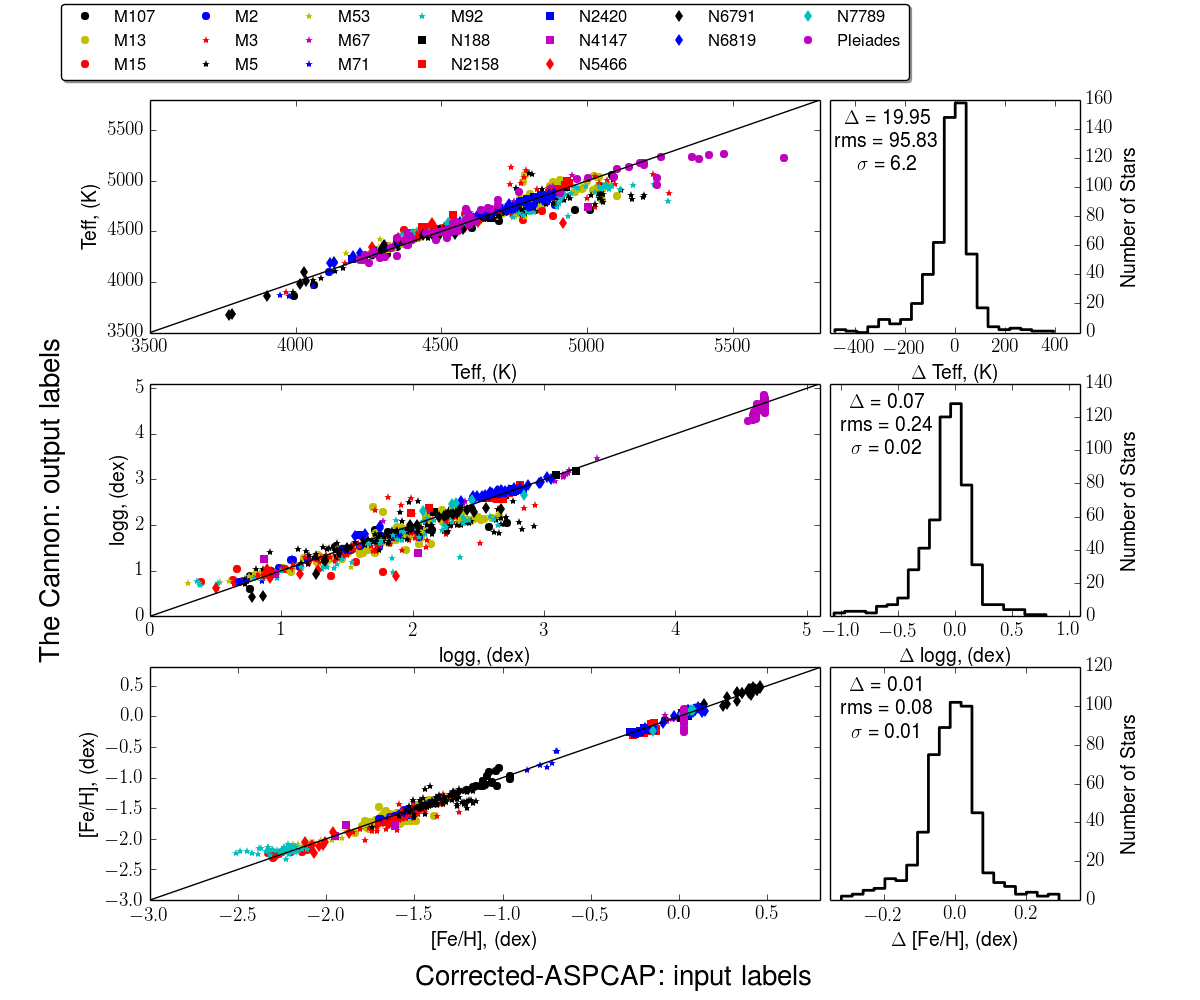
\includegraphics[scale=0.45]{./plots/takeout_histc.png}
\caption{The take-one-star-out cross-validation of the 543 stars in the training dataset using the quadratic model in equation~(\ref{eq:quadinthreelabels}) and corresponding histograms at right, showing \tc\ output -- \apogee\ input labels.}
\label{fig:takeonestarout}
\end{figure}
%\begin{figure}[h!]
%\centering
%  \includegraphics[scale=0.45]{./plots/mkn_labels.pdf}
%\caption{Take-one-star-out cross-validation of the 530 stars in the training dataset with own-labels}
%\label{fig:takeonestarout_own}
%\end{figure}

The outlying stars in \figurename~\ref{fig:takeonestarout} may be due to an anomalous scale of the input labels of these stars compared to the other training data, or it may be a consequence of the model being too inflexible to properly model how flux changes with labels across the parameter space of the training dataset. 
The temperature of the dwarfs is offset low at increasing temperature, compared to the input labels, so the model may be limited in describing the difference between dwarf and giant spectra. 
There is a flattening at the low metallicity end of the model in \feh\ in the output labels at \feh\ $<$ -2.2, however this value of \feh\ = --2.2 also corresponds to the literature value of this cluster, M5 \citep{Meszaros2013}. 
The lower metallicity of the \aspcap\ label may represent internal scatter in the \aspcap\ results.
The fact that \figurename~\ref{fig:takeonestarout} shows only very small systematic offsets and such tight scatter leads us to conclude that for the
current context the quadratic-in-labels spectral model is sufficient in the label tranfer. 

Interestingly, an analogous take-one-cluster-out test significantly increases the scatter in the label transfer, 
increasing the rms differences to $<$ 150 K in \teff, $<$ 0.4 dex in \logg\ and $<$ 0.12 dex in \feh.
This indicates that our training set is sufficiently small that each cluster matters for a good label transfer. 
One particular case in the \apogee\ context is the Pleiades cluster: it is the \textit{only} cluster for which dwarf stars have been observed and hence we can draw reference labels for main sequence stars. 
 
We now turn to illustrating where the information that led to the accurate label transfer (\figurename~\ref{fig:takeonestarout}) came from in the spectra.
\figurename~\ref{fig:coeffs} shows -- across the narrow regions (A) and (B) of the spectra, marked in \figurename~\ref{fig:norm} -- the first coefficient vectors $\theta_{0,1,2,3}$ of the spectral model (those linear in the three labels), which were fit in the training step for the quadratic-in-labels model in equation~(\ref{eq:quadinlabels}). 


The top panel shows the zeroth order-coefficient vector $\theta_0$, or the baseline spectrum, of the model. 
The mid panel shows the coefficients that are simply linear in \teff, \logg\ and \feh.
In the top panel of \figurename~\ref{fig:coeffs}, the red, blue and green shaded wavelength regions with the 5\% 
highest coefficient values $|\theta_{1,2,3}|$ in the \feh, \teff\ and \logg\ labels respectively. 
These regions indicate where the spectra's flux levels strongly vary with these labels.
This also highlights that different parts of the spectrum depend differently on the labels. Note there are many regions where the \feh\ label dominates in contribution to the flux.
For the first label vector for example in the middle panel of \figurename~\ref{fig:coeffs}, 
there is typically asymmetry for a given absorption feature, in the flux and the labels. 
There are very few regions where the flux is a function of only one of the labels, and pixels are typically covariant 
(that is, the same pixel will have a higher flux at both lower \teff\ and higher \feh). 
This simply reflects well-known covariances between, for example, temperature and \feh .
The strongest \logg\ dependence is typically associated with weak lines including the wings of the 
feature and the \feh\ label, with strong lines, particularly the depth of the line. 

The bottom panel of \figurename~\ref{fig:coeffs} shows the scatter vector of the spectral model, 
indicating the dispersion of the flux of the training data around the best-fit spectral model at each pixel. 
The scatter is small and this indicates that our model is a good representation of the data. 
However, the scatter is highest where the most information in the spectra are contained. 
This implies that either our quadratic-in-labels spectral model is still somewhat too restricted, or that the labels of our training dataset are imperfect or incomplete 
(for example, lacking $[\alpha / Fe]$ as a label), or a combination of these effects. 
From the coefficients of an initial fit of this spectral models (see, for example, the middle panel of \figurename~\ref{fig:coeffs}), 
the continuum pixels have been determined following \sectionname~\ref{sec:ContNorm}. 
These are marked in the black dots in the top panel of the \figurename, and are used for an iterated, 
consistent continuum normalisation for all spectra, both of the reference and of the survey objects.

%+\textbf{HWR: }\texttt{If that is the place where we praise, based on practical examples, the advantages of \tc\ vis-a-vis hand-defined \textit{indices} of physical models, it should be more extensive... else, defer to discussion. - moved the paragraph on \tc\ being a tool to return coefficients so a full model - to the discussion} 

  %made with run -i makeplot_scatter_test18_step_revc.py
\begin{figure}[h!]
\centering
    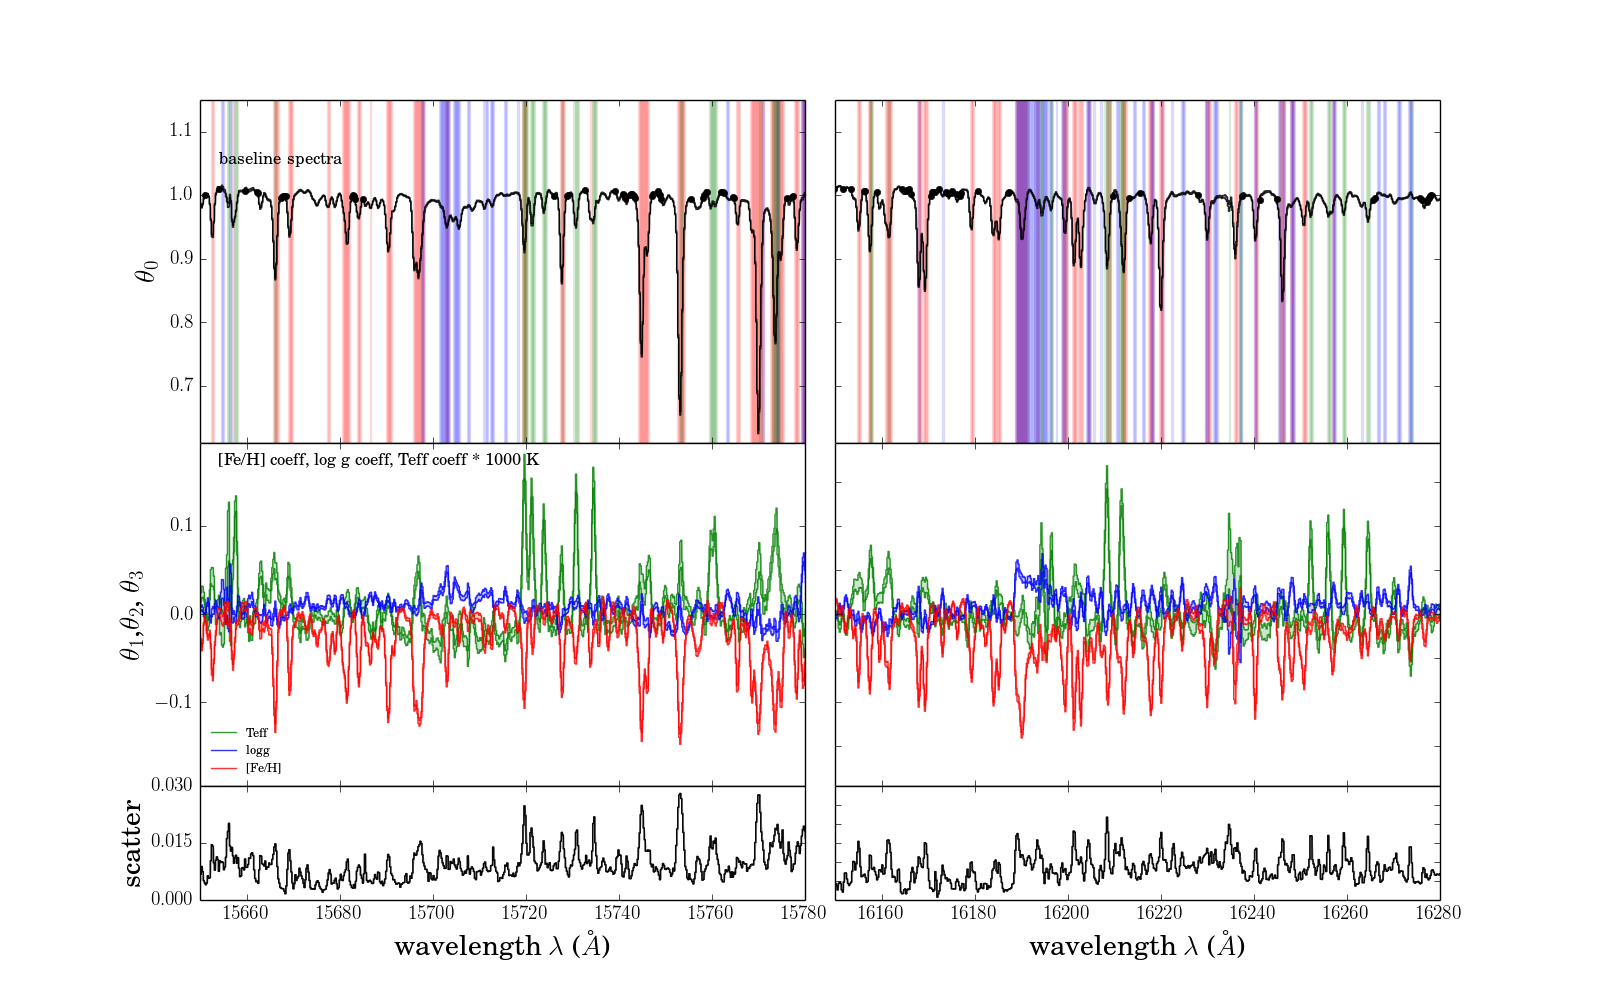
\includegraphics[width=\hsize]{./plots/R1_continuum5.png}
  \caption{The first-order coefficients and scatter across the sample regions of the spectra from \figurename~\ref{MKNFIXME}, A and B. Top panel: the baseline spectra representing the first coefficient from the set of reference spectra; middle panel: the next three coefficients ($\theta_1$, $\theta_2$, $\theta_3$),  which correspond to the labels ($\teff, \log, \feh$); bottom panel: the scatter of the fit with a tenfold expanded vertical scale.  The red, blue and green areas in the top panel encompass the wavelength regions with the 5\% highest (absolute value) coefficients for the \feh, \teff\ and \logg\ labels respectively. This indicates where the flux in these spectrum is particularly sensitive to the labels.  Note the \feh\ label is dominant in the contribution level and from the top panel it is clear that there is significant covariance between the labels and there are only a few regions of \logg\ sensitivity. The filled dots in the baseline spectrum in the top penal indicate the wavelengths at which the dependencies on all labels are weak, which we operatively identify as continuum pixels (see \sectionname~\ref{MKN REF}).}
\label{fig:coeffs}
\end{figure}
\textbf{We had once talked about scaling these coefficients - how do I do this exactly - x mean/range? Note to HWR - This is the first order coefficients for the quadratic model, I can use the simple first order model to make this (which the changes to the caption in the marked up pdf are consistent with doing) but the scatter is higher - let me know which is preferable.}

\textbf{DWH: caveat about our cross-validation and signal to noise}. 

\subsection{Identification of \apogee\ Continuum Pixels}
\label{sec:ApogeeContinuum}

The continuum pixels, which are shown in \figurename~\ref{fig:coeffs} for wavelength regions A and B, 
have been determined from the quadratic model using a combination of the flux level and the coefficients returned
(cf. \sectionname~\ref{sec:ContNorm}). Specifically, we found that 35\% of the pixels in the baseline spectrum of the model (the vector $\theta^0_\lambda$) flux levels within 1\% of unity. However, not all these pixels are suitable continuum pixels, as many of them have significant dependencies (that is, $\theta^{1,2,3}_\lambda$)
on the three labels. 
In practice, we make a continuum selection taking the 15\% of pixels with coefficients nearest 0 for each coefficient and a flux selection of 1 $\pm$ 0.15 [{\bf HWR: really $\pm$ 15\% ? I thought 35\% are within 1\% ?, MKN - they are this is just what worked well - I can redo some tests of this.}]
These criteria return around 7\% of pixels, which we adopt as true continuum pixels for data that span the label range of the training set. We use the inverse variance weighting of these pixels for the corresponding 2nd order Chebyshev polynomial fit. 
As we show explicitly in \sectionname~\ref{sec:lowSNR}, we find this to provide a robust continuum normalisation across the stars that are within the parameter range of the training set, 
across all SNR. 

\subsection{\tc 's Label Transfer for \apogee\ DR10}
\label{sec:APOGEE_DR10_comparison}

Going beyond leave-one-out tests on the set of reference objects, we now apply \tc\ to effect a label transfer to the entire \apogee\ DR10.
We take the spectral model built in the \apogee\ cluster stars in \sectionname~\ref{sec:ModelComplexity}, \sectionname~\ref{sec:take-one-out} and \sectionname~\ref{sec:ApogeeContinuum},
and apply the test step with this model to all DR10 spectra.
Remarkably, we are able to reproduce well the \aspcap\ labels for DR10 spectra. We have run \tc\ through all 47,000 stars in 150 fields in DR10 contained in the available \textit{aspcapstar} files as well as an additional 4800 stars in 20 commissioning fields for which no \aspcap\ parameters were provided in DR10, 
made available in the (non pseudo-continuum normalised) \textit{apStar} files. 
We also have run \tc\ through the additional commissioning stars available in the \apstar\ files across the fields and in total this
 comprises 55,000 DR10 stars in 170 fields. %These 170 fields comprise a total of $\sim$ 51,600 \apogee\ DR10 stars. 

These results of \tc\ for all DR10 stars for which we return parameters are provided online in \tablename~\ref{tab:online}. 
For the 30,500 stars with parameters provided by DR10, we find we reproduce the \apogee\ labels as follows: 
\teff\ = +12 K $\pm$ 87 K , \logg\ = --0.04 dex $\pm$ 0.18 dex and \feh\ = +0.01 $\pm$ 0.10 dex in \feh. 
The rms errors are comparable to the error estimates for \apogee\ parameters in \citet{Meszaros2013} 
of $\delta$(\teff) $<$ 150 K, $\delta$(\logg) $<$ 0.2 dex and $\delta$(\feh) $<$ 0.1 dex in. 
The typical internal precision on the measured parameters from \tc\ is $\delta$(\teff) $<$ 5.6 K, $\delta$(\logg) $<$ 0.01 dex and $\delta$(\feh) $<$ 0.006 dex.

\begin{table*}[!h]
\small{
\centering
\caption{Excerpt from full online version of table of parameters for the 55,000 stars released in 170 fields from \apogee\'s data release DR10. Stars with rotation warning = 1 flag set have unphysical stellar parameters and commissioning stars are marked with ``C'', the fidelity of the commissioning stars is uncertain given their different LSF from survey test and training data.} \begin{tabular}{| c | c | c |  c | c | c |  c | c | c |} %51,500
\hline
star ID & \teff\ & \logg\ & \feh\ & $\sigma$(\teff) & $\sigma$(\logg) & $\sigma$(\feh) & $\chi^2$ & \tiny{ROT WARN}\\
{2MASS} &  K &  dex  & dex & K & dex & dex & & \\    
\hline
%21353892+4229507 & 4131.7 &  1.51 & 0.04 & 3.25 & 0.0116 &  0.0042 & 11.06 &  0.0\\
21354474+4250256 & 5028.5 & 4.53 & 0.13 & 9.14 & 0.01 & 0.006 & 3.14 & 0\\
21354775+4233120 & 4730.9 & 2.8 & 0.06 & 12.02 & 0.04 & 0.011 & 1.34 & 0\\
21355458+4222326 & 4780.1 & 2.42 & --0.36 & 8.34 & 0.03 & 0.007 & 2.41 & 0\\
21360285+4231145 &  4552.4 &  1.96 & --0.46  & 10.83 & 0.04 & 0.011 &  1.42 &  0\\
 \hline
\end{tabular}
\label{tab:online} }
\end{table*}  
 
The comparison of \tc\ with ASPCAP, showing the bias, rms and formal precision for the labels (\teff , \logg , \feh ) in six sample fields, with bulge, disk and halo targeting, is illustrated in \figurename~\ref{fig:cal}. As for all stars in the survey with \aspcap\ labels, these fields show that we reproduce the \aspcap\ corrected stellar parameters with typical rms uncertainties of \teff\ $<$ 100 K, \logg\ $<$ 0.20 dex and $<$ \feh\ $<$ 0.10. These variances are slightly smaller than expected from our cross-validation leave-one-star-out test. This may be because the median of the stellar labels for the D10 survey object are near the median labels of the reference objects from the training step. 
They are not concentrated to the extreme ends of the range, which have a higher weighting in evaluating the test data with cross validation. 
The \tc 's label transfer also returns values for those +15\% of stars in DR10 are that must be main-sequence dwarf stars. 
These are not shown in \figurename~\ref{fig:cal}, as \apogee\ does not report ASCAP corrected dwarf parameters for DR10. 
We exclude the rapid rotators using the \aspcap\ \rotwarn\ flag as we can not return parameters for spectral types not included in our training set (see \sectionname~\ref{sec:AnomalousSpectra}). 

In \figurename~\ref{fig:cal} we show the label differences of \tc\ $-$ \aspcap\ for the 1400 stars from the six sample fields as a function of \aspcap\ \teff, \logg\ and \feh. There are weak trends; at low \teff\ $\sim$ 3700 K, we find temperatures about 100 K cooler than \apogee\, at low \logg\ we find $\sim$ 0.15 dex larger \logg\ than \apogee\ and at the lowest metallicities \feh\ $<$ --2.0, we typically report higher metallicities on the order of 0.05 to 0.3 dex.


%makeplot_fits_v19_bw.py
\begin{figure}[!h]
\centering
  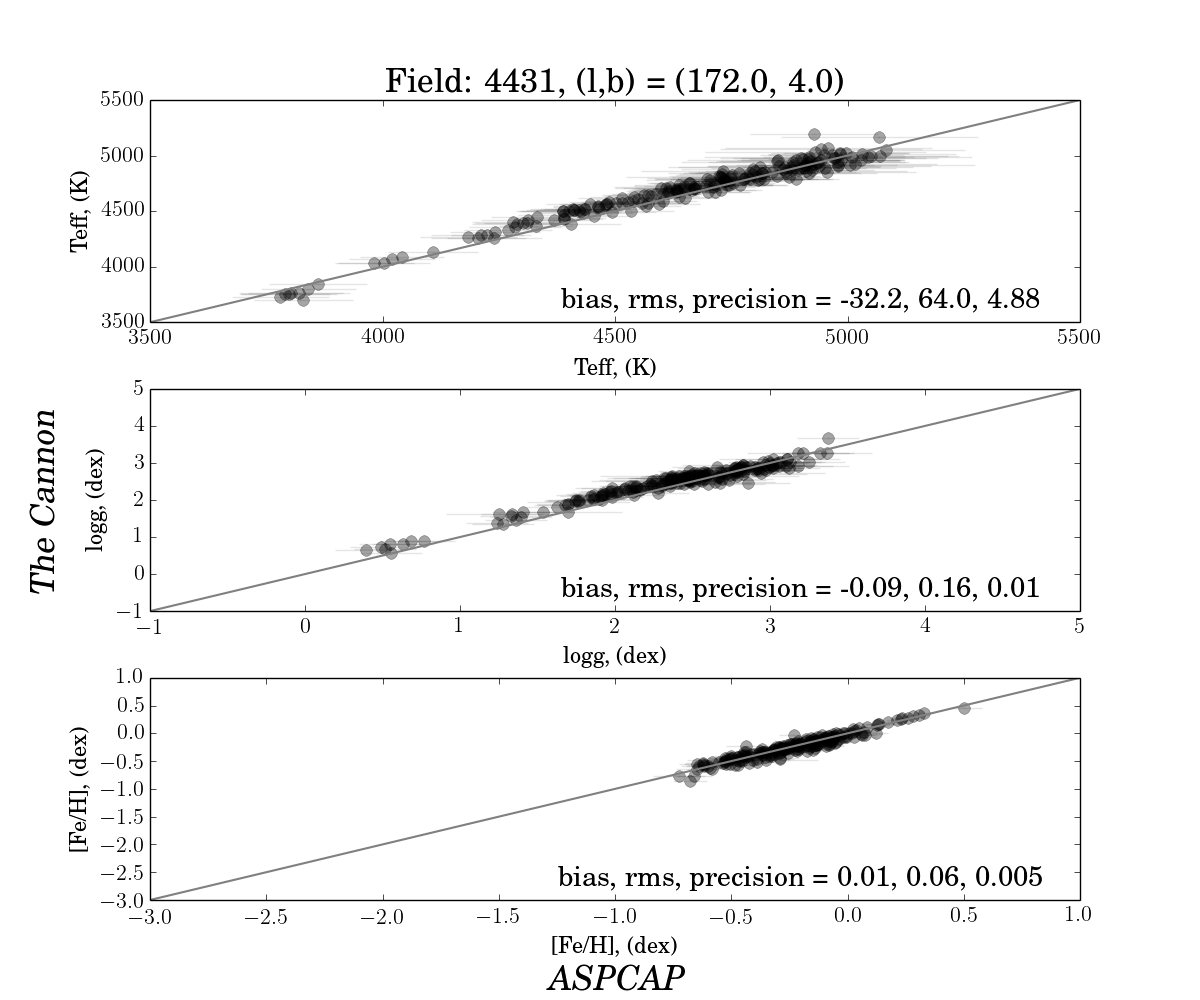
\includegraphics[scale=0.23]{./plots/4431_v19.png}
    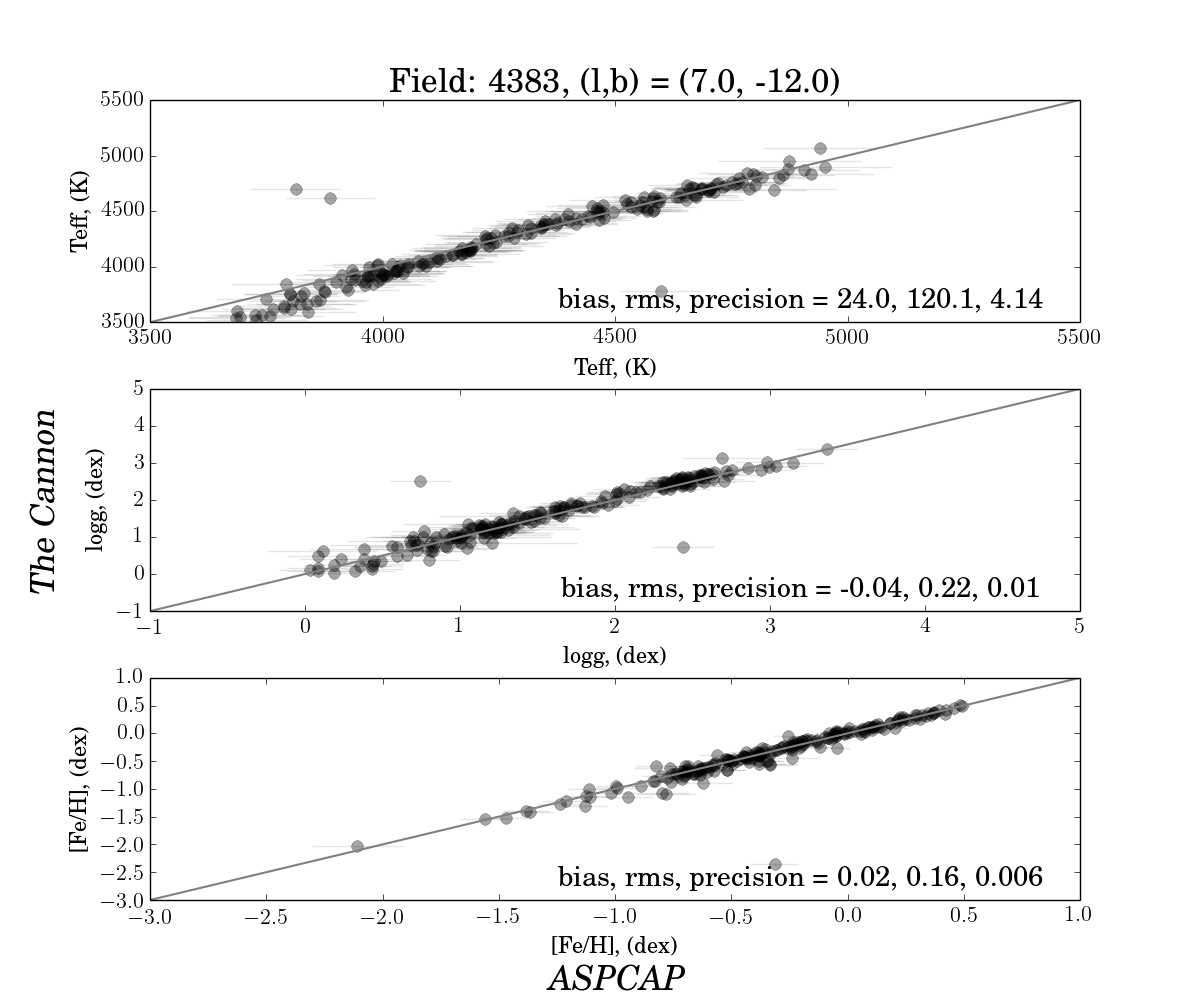
\includegraphics[scale=0.23]{./plots/4383_v19.png} \\
      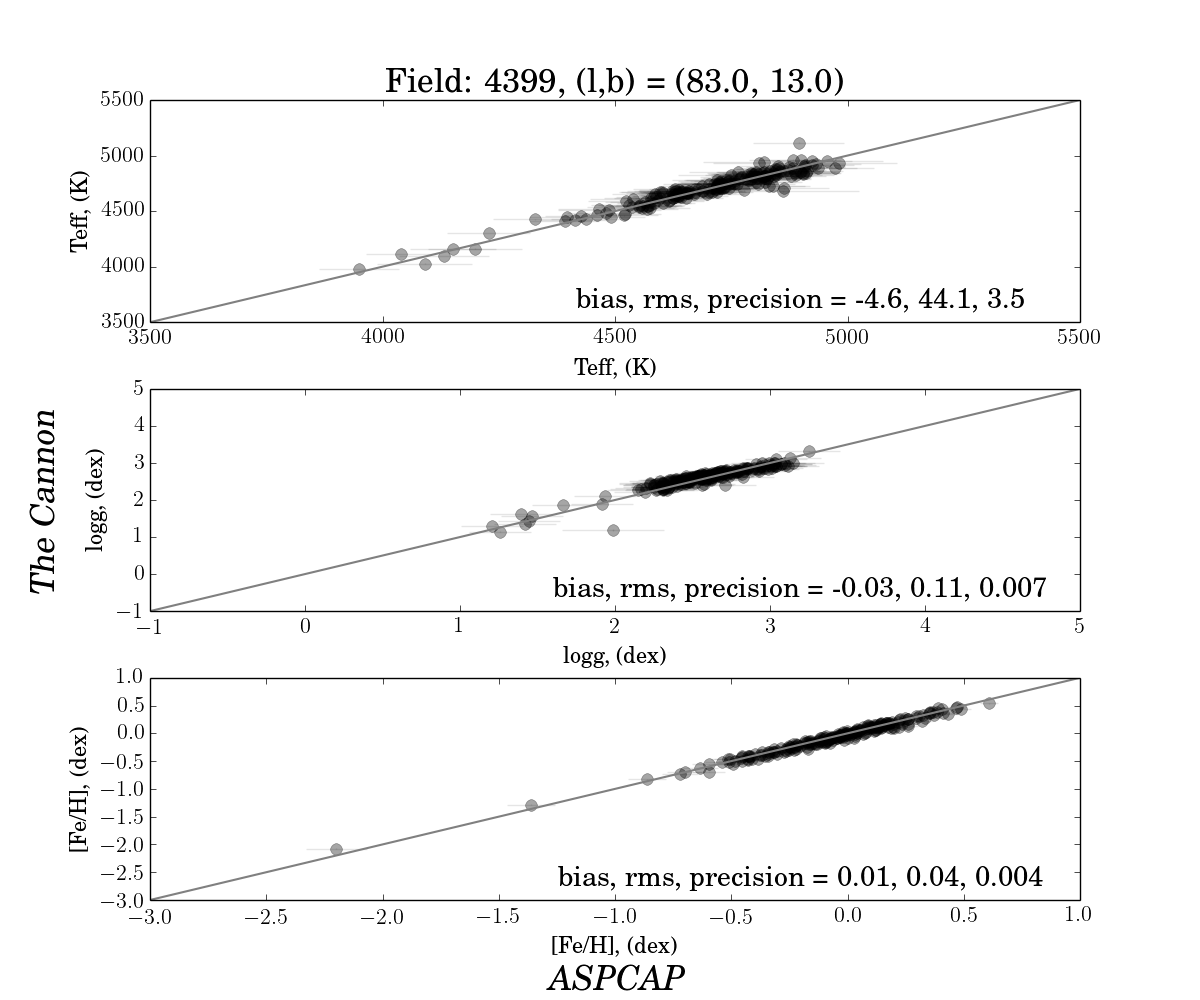
\includegraphics[scale=0.23]{./plots/4399_v19.png}
        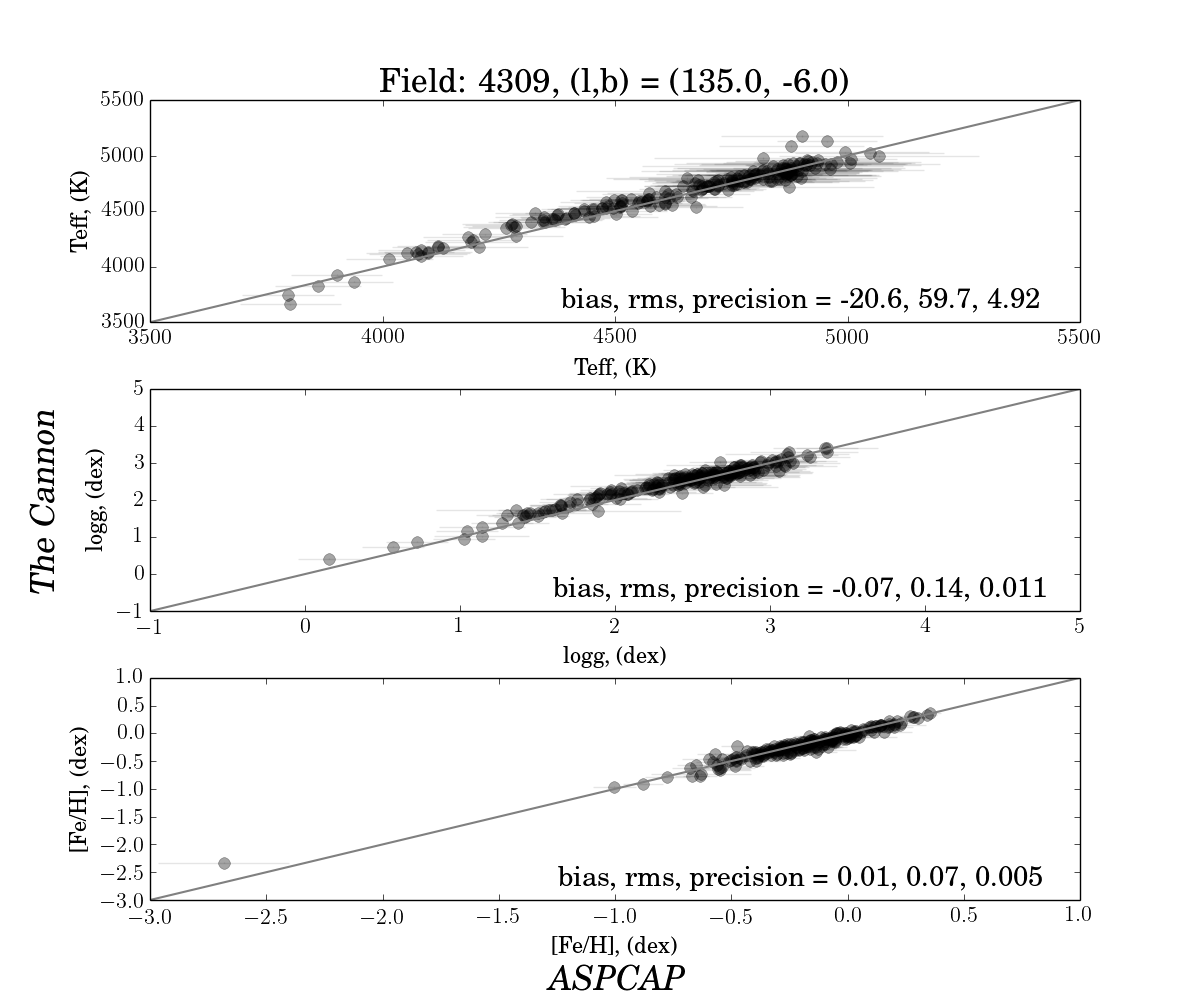
\includegraphics[scale=0.23]{./plots/4309_v19.png} \\
              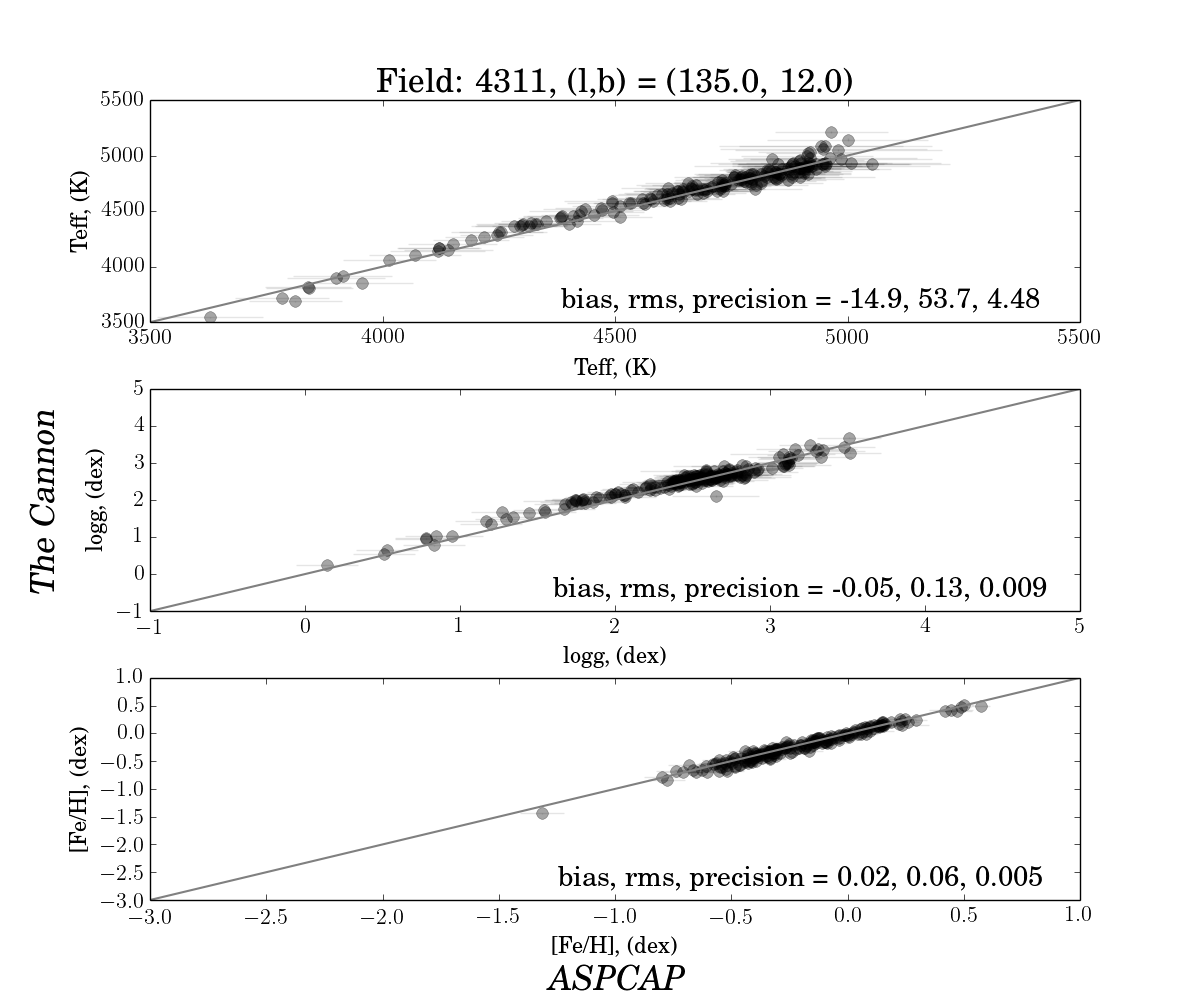
\includegraphics[scale=0.23]{./plots/4311_v19.png}
        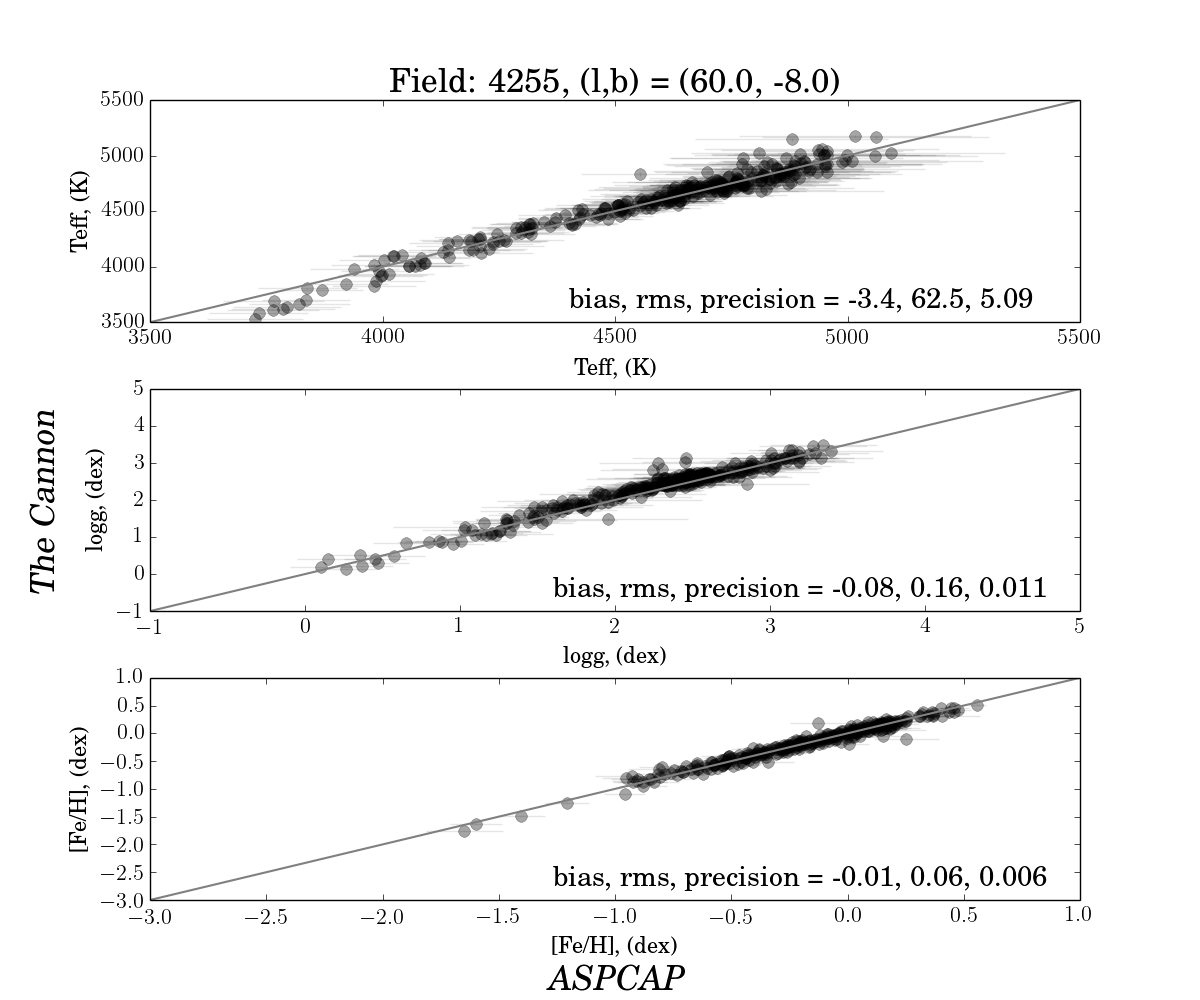
\includegraphics[scale=0.23]{./plots/4255_v19.png} 
\caption{\small{\aspcap\ DR10 versus \tc\ for six different fields including in the disk, bulge and halo. The number of stars is, for each subfigure is 211 (4431), 207 (4384), 217 (4399), 210 (4309), 198 (4311) 319 (4255) }}
\label{fig:cal}
\end{figure}

%run -i makeplot_fits_v19_3by3c.py with plotfits_v19('listin.txt')
\begin{figure}[!h]
\centering
        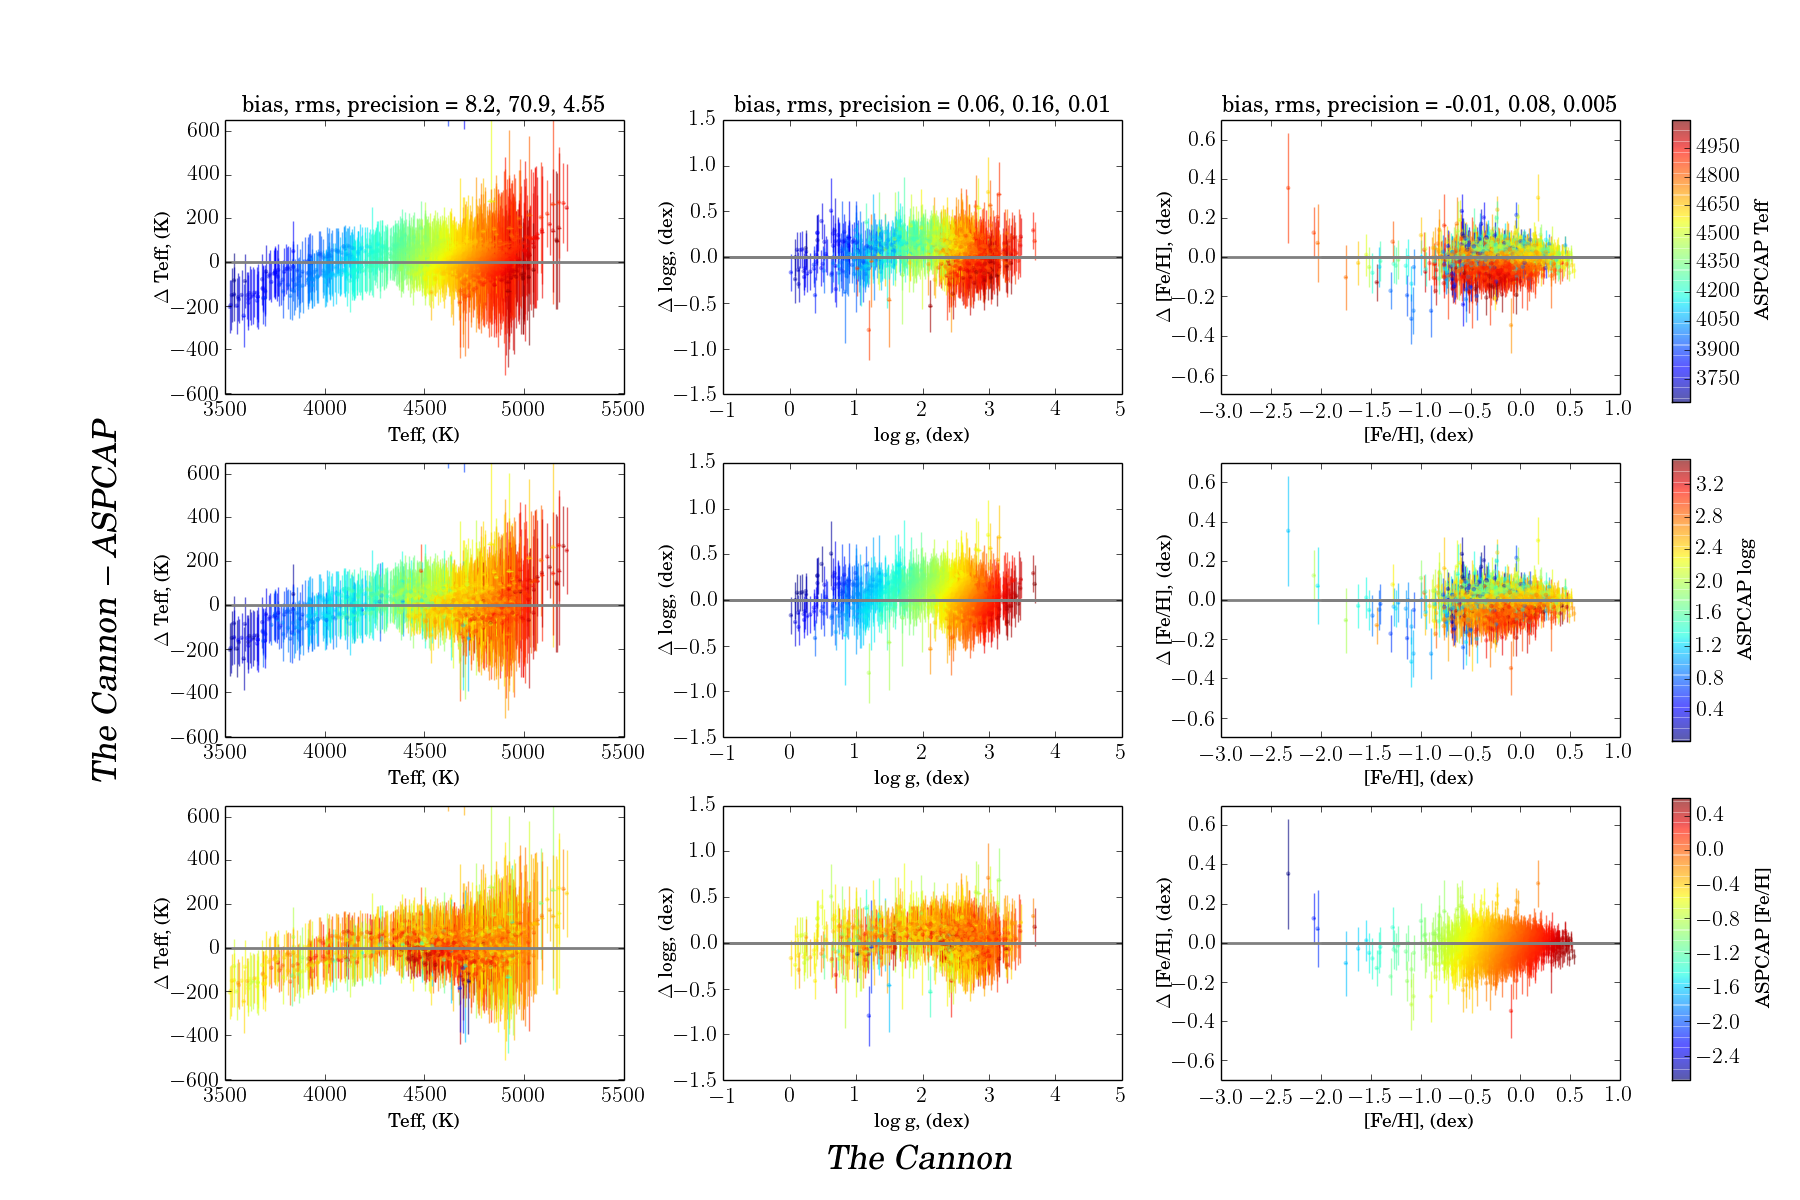
\includegraphics[scale=0.35]{./plots/cplot2.png} 
\caption{Difference between the labels (\teff, \logg, and \feh) derived through \tc\ in the test step and their \aspcap\ DR10 values for all the 1400 stars shown in \figurename~\ref{MKNFIXME}. The error bars are dominated by those quoted by \aspcap. There are systematic offsets at the coolest temperatures.}
\label{fig:cplot}
\end{figure}


We show \tc 's resulting label distribution in the \teff-\logg\ plane from \tc\ for the stars in DR10 in \figurename~\ref{fig:iso}. 
This \figurename\ shows the result when \aspcap -corrected labels labels are used for the reference objects in teh training step; \figurename~\ref{fig:iso2} shows the analogous results but for isochrone-corrected reference labels. There are 37,500 stars in these \figurenames\ that are remain after excluding stars with the \rotwarn\ flag set, with velocity scatter $>$ 10 \kms\ and telluric calibration target set. These \figurenames\ also show the labels for the 15\% stars with \logg $>$ 4 dex that must be main sequence stars.
 Only the stars that have been determined using targeting flags and inspection of the spectra to be dwarfs with rotation, 
 have been removed using the \aspcap\ rotation warning set flag. 
 Were we to force label transfer with \tc , we find that the labels lie an unphysical space at very low \feh and \logg and high \teff.

In short, for all stars with good \aspcap\ labels, we find excellent agreement between \tc\ and \aspcap\ by adopting ASCPAP corrected labels in the training step.
In addition, we are able to derive plausible parameters for dwarf stars in DR10. However, the \teff-\logg\ plane for these stars shows a deviation from the giant branch of the isochrone at low \logg\ (see the right panel of \figurename~\ref{fig:iso}). This is a consequence of the input labels of the training spectra. 

If instead we use the isochrone-corrected \logg\ labels to fix \tc 's spectral model
(cf. \sectionname~\ref{sec:ReferenceObjects}), the results of the label transfer deviate slightly from the \aspcap\ scale in each of the parameters. 
However, with these new \logg\ labels, we find a broad giant branch width that is consistent with expectations in \teff-\logg\ space 
given the metallicity of these stars (see the right hand panel of \figurename~\ref{fig:iso2}). 

This comparison again illustrates both the power of \tc\ to transfer labels, but also its dependence on the choice of suitable reference labels. 

Currently, no priors are incorporated in the \tc\ to place the resulting label estimates near physically plausible isochrones. 
Nonetheless, almost all stars lie in physical spaces on the isochrones as shown in \figurenames~\ref{fig:iso} and \ref{fig:iso2} validates the labels. 
The labels for the main sequence stars are presumably much more poorly determined, given the limitations of the reference objects in the training step. 
Remarkably, though, only a handful of stars at low \feh\ and low \logg\ do not lie near conceivable isochrones. 

At metallicities \feh\ $<$ --0.25 the red clump is offset too high in the \logg\ label. This is noted in \citet{bovy2014} who estimate that this offset shifts the red clump and red giant branches 0.2 dex closer together. 
Our \logg\ labels in \figurename~\ref{fig:iso} are essentially identical to \apogee\ ASPCAP labels (offset -0.04 dex in \logg\ for DR10) and the left panels show that the red clump stars which should be seen as a density maxima of stars around \logg\ $\sim$ 2.5, \teff\ $\sim$ 4800K \citep[e.g.,][]{Zhao2001} 
are offset to higher \logg\ than the red clump branch of the Padova isochrone, for stars \feh\ $<$ --0.25. 
This offset is on the order of 0.2 dex at \feh\ = -0.5 and is present for both \aspcap-corrected labels and isochrone-corrected labels. 
This may indicate that the \aspcap\ temperature scale is offset too cool in DR10 (but as a function of \feh).

%\textbf{have written -find it odd this is not discussed in Jo Bovy's paper: note to MKN: Discuss that red clump is not where it should be for stars $<$ --0.25, Jo Bovy didn't show this in the paper but does mention there is a systematic offset - it's pretty bad though - instead shows apocask stars on the padova isochorne fit. This plot/discussion never appears in apogee papers - is it just as one wants to project the positive aspects and not all aspects of the results that this has been omitted or am i just missing a of it elsewhere?}.

% made with makeonisochrone_v18_bw.py
\begin{figure}[!h]
\centering
  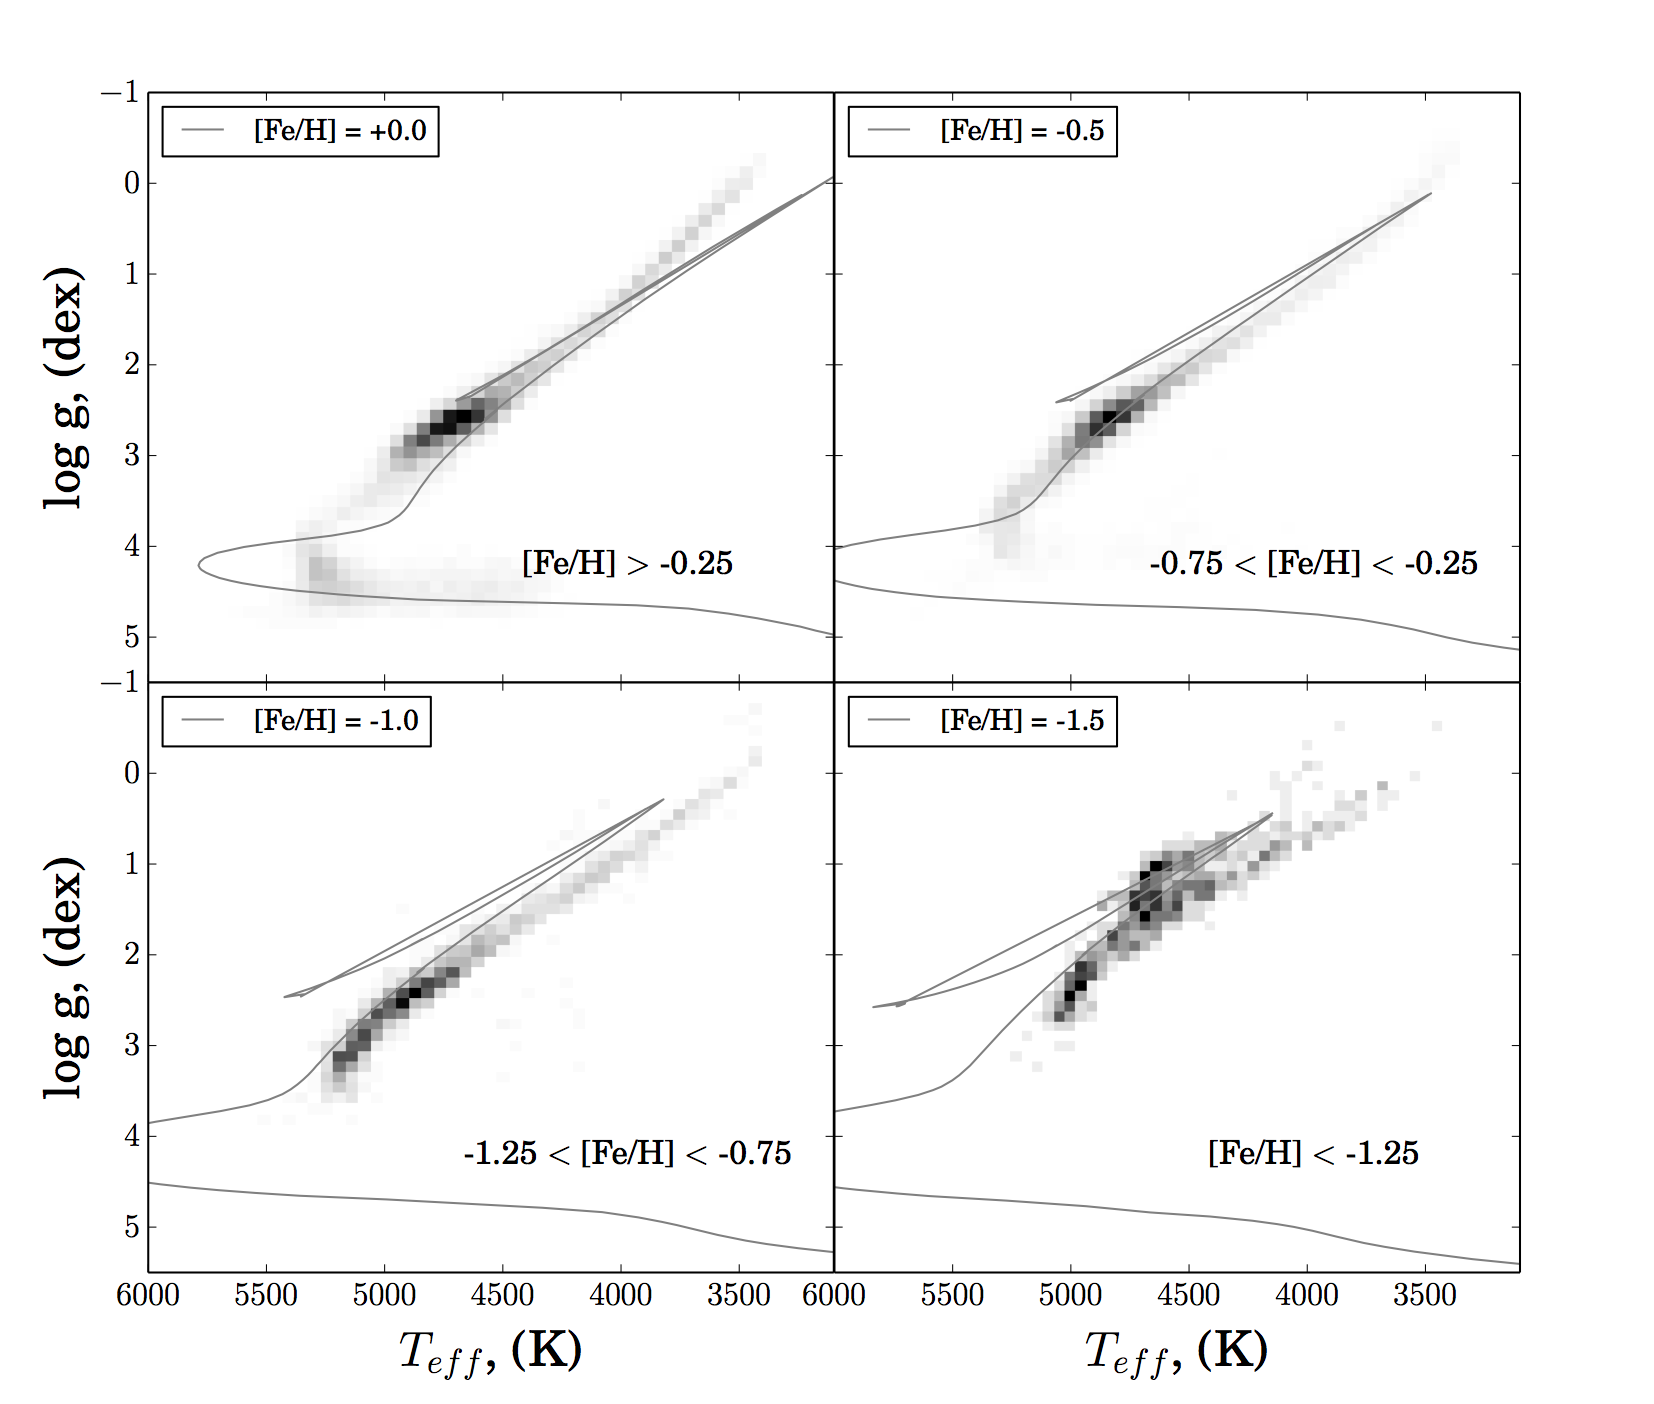
\includegraphics[scale=0.25]{./plots/iso1.png}
  \hspace{-20pt}
    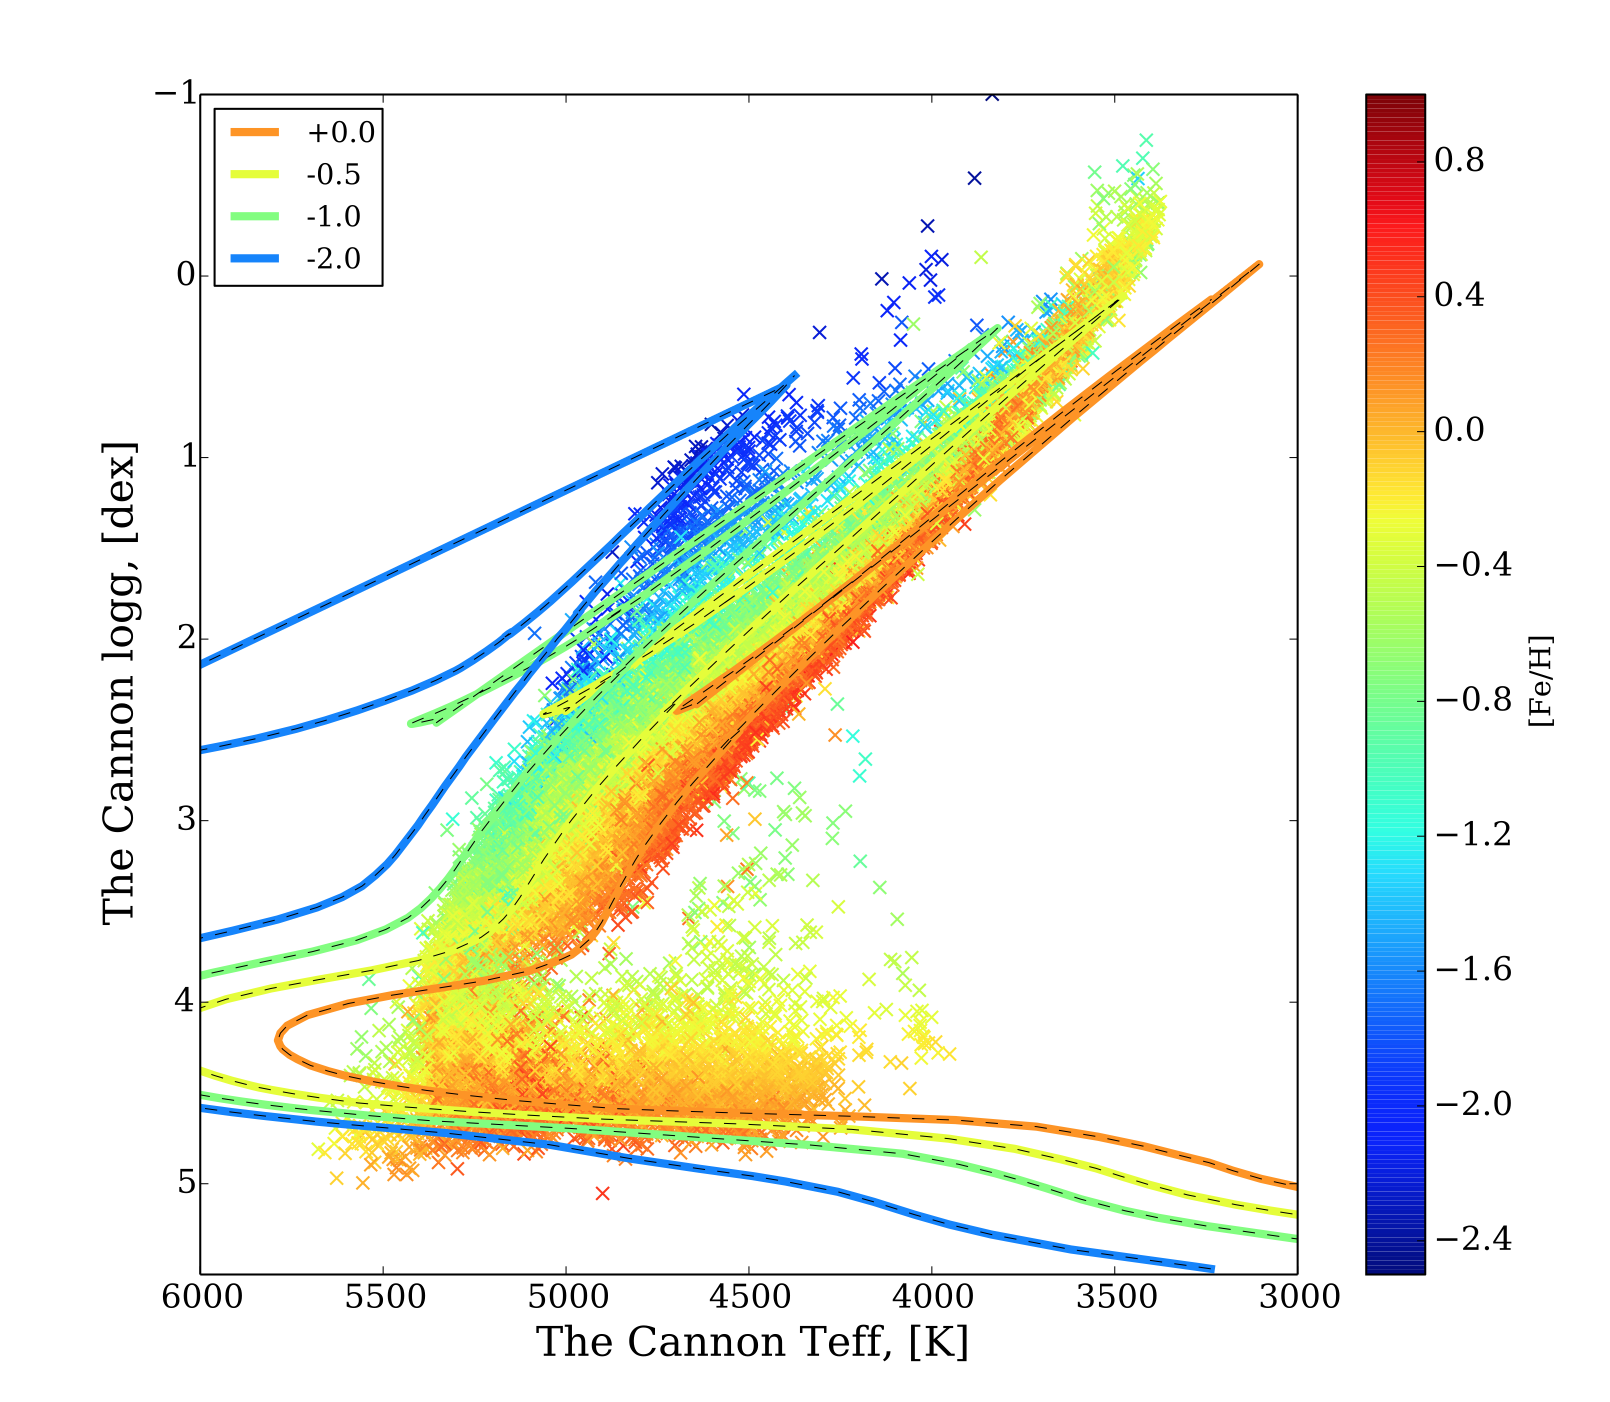
\includegraphics[scale=0.25]{./plots/iso1a.png}
%    \includegraphics[scale=0.33]{./plots/isochrone_mkn20b2.pdf}
\caption{Labels for the $\sim$ 38,000 stars from DR10 derived by \tc\ based on \aspcap-corrected labels for the set of reference objects. The set of panels on the left shows \teff-\logg\ in four metallicity bins. There are $\sim$ 21,600, 14,000, 1700, and 900 stars in the most metal-rich to metal-poor metallicity bins, respectively. The isochrones plotted are 10 Gyr Padova isochrones at the metallicities marked in the upper left hand corners of each sub-panel.  The panel on the right shows all stars coloured in \feh\ on the four isochrones. Note the \logg\ distribution at low \logg\ is narrow and offset from the giant branch. }
\label{fig:iso}
\end{figure}


\begin{figure}[!h]
\centering

      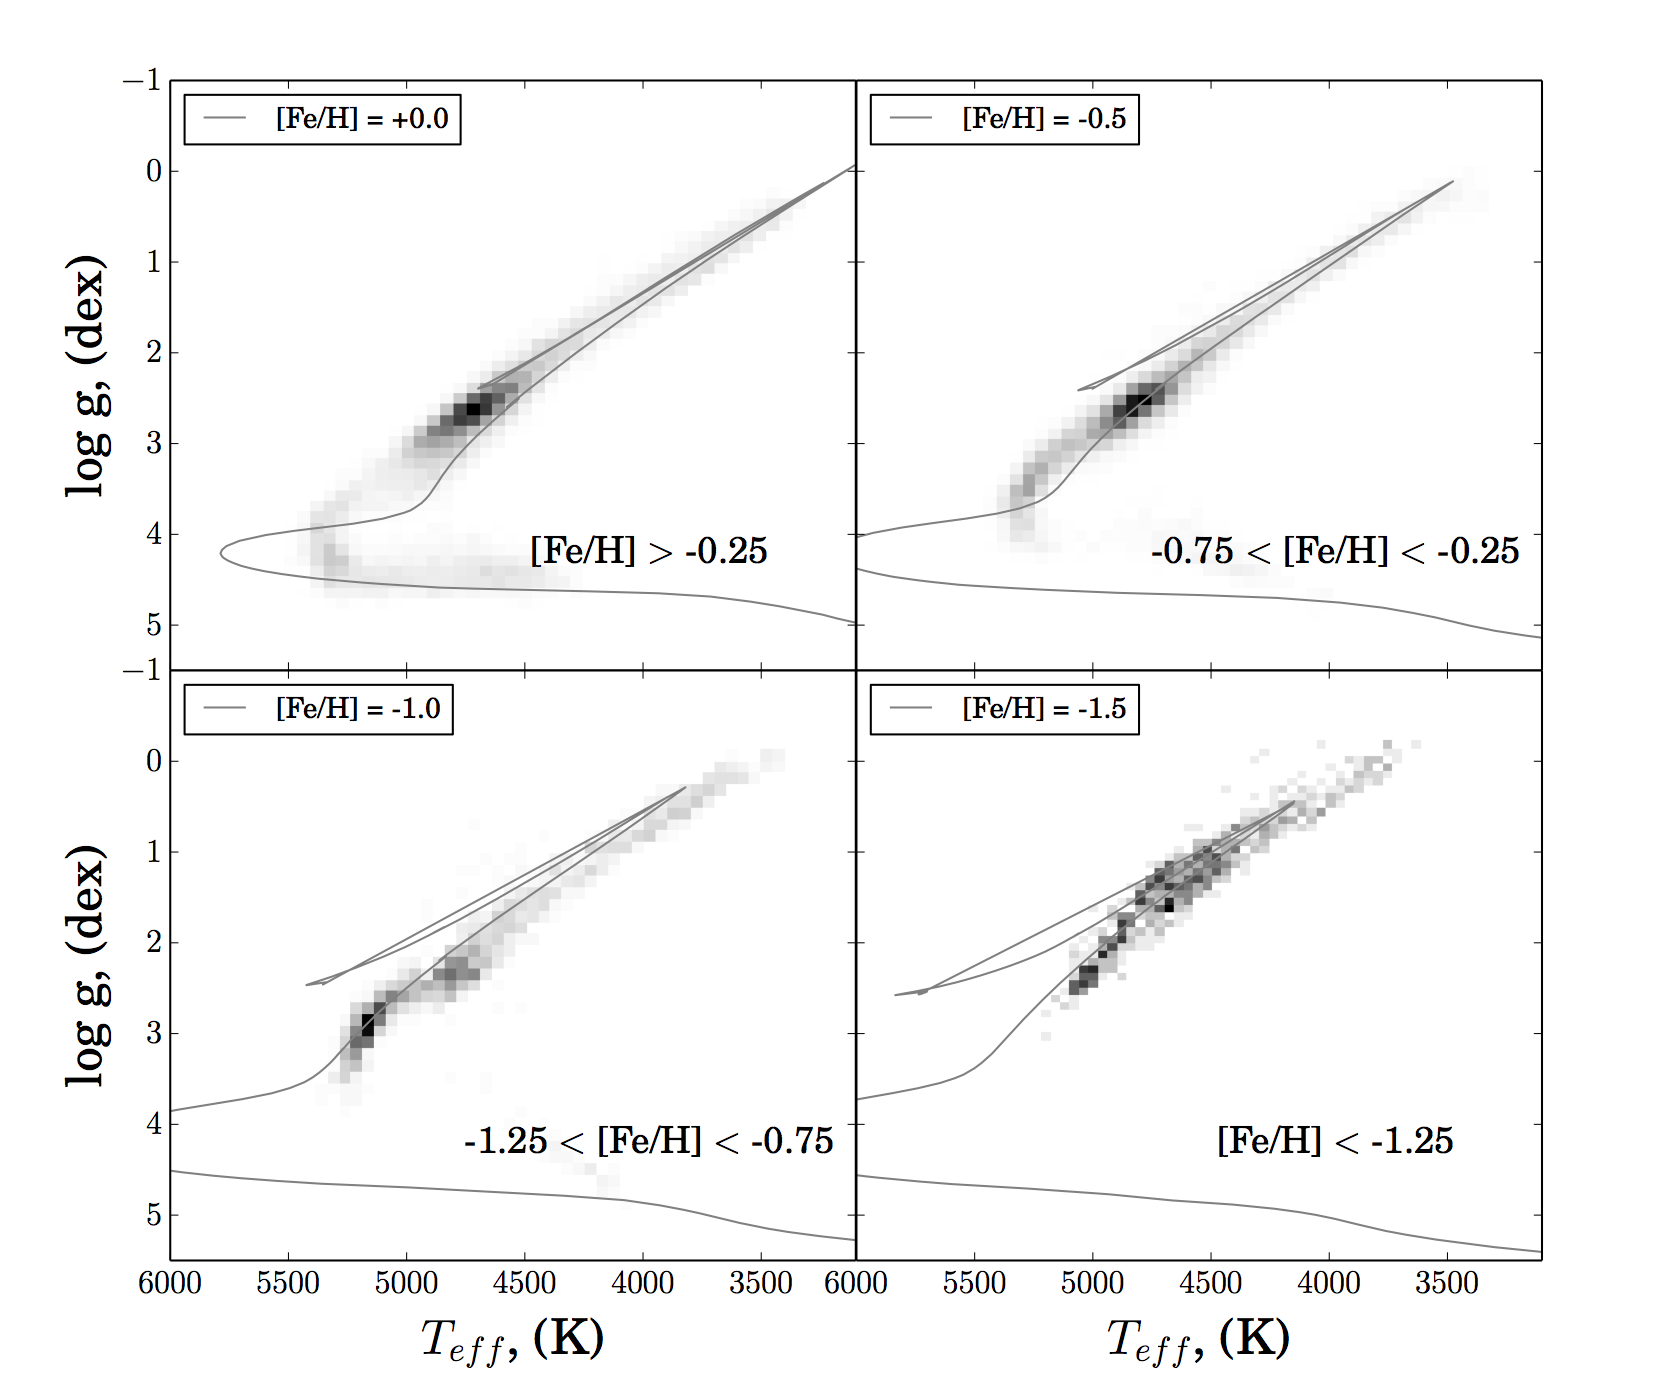
\includegraphics[scale=0.25]{./plots/iso2.png}
  \hspace{-20pt}
    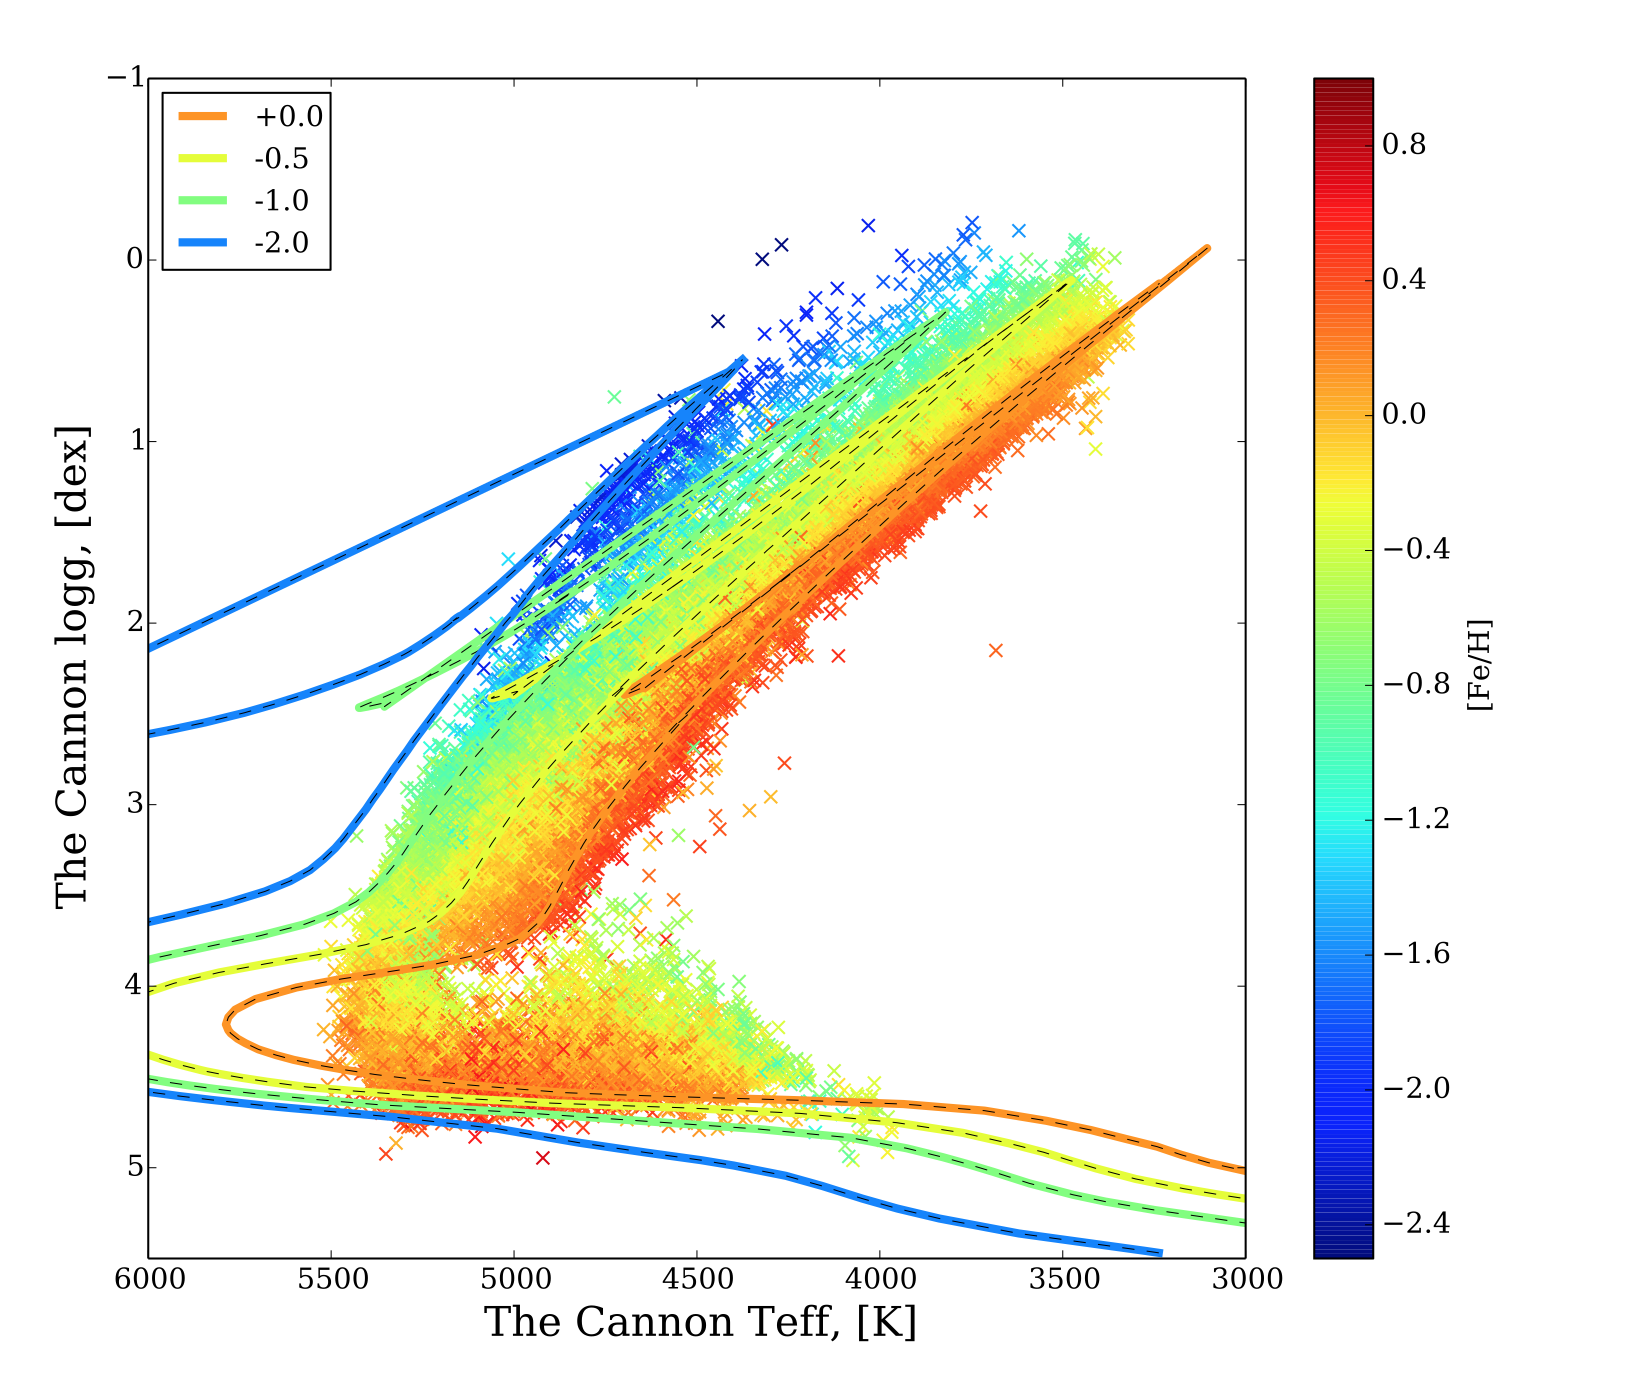
\includegraphics[scale=0.25]{./plots/iso2a.png}
%    \includegraphics[scale=0.33]{./plots/isochrone_mkn20b2.pdf}
\caption{Same as \figurename~\ref{fig:iso} but based on the isochrone-corrected'' labels for the reference objects. In this case, the labels follow the red giant branch on the isochrones. Note that there is nothing in the mathematics of \tc\ (\ref{eq:10}) that forces resulting labels to lie in physically plausible location sod label space. This is illustrated by the tiny fraction of objects that lie between the main sequence and the giant branch. That most labels lie in physically sensible portions of the \teff-\logg\ plane is a testament to both the quality of the label coverage in the set of reference objects and to the power of \tc\ approach. This is all the more remarkable as there are basically no main sequence stars among the reference objects.}
\label{fig:iso2}
\end{figure}


\subsection{Failures: Types of Spectra not Represented among the Reference Objects}
\label{sec:AnomalousSpectra}

 %run -i makeplot_scatter_test18_coeffs_dwarfs_RevB.py
  \begin{figure}[!h]
   \centering
 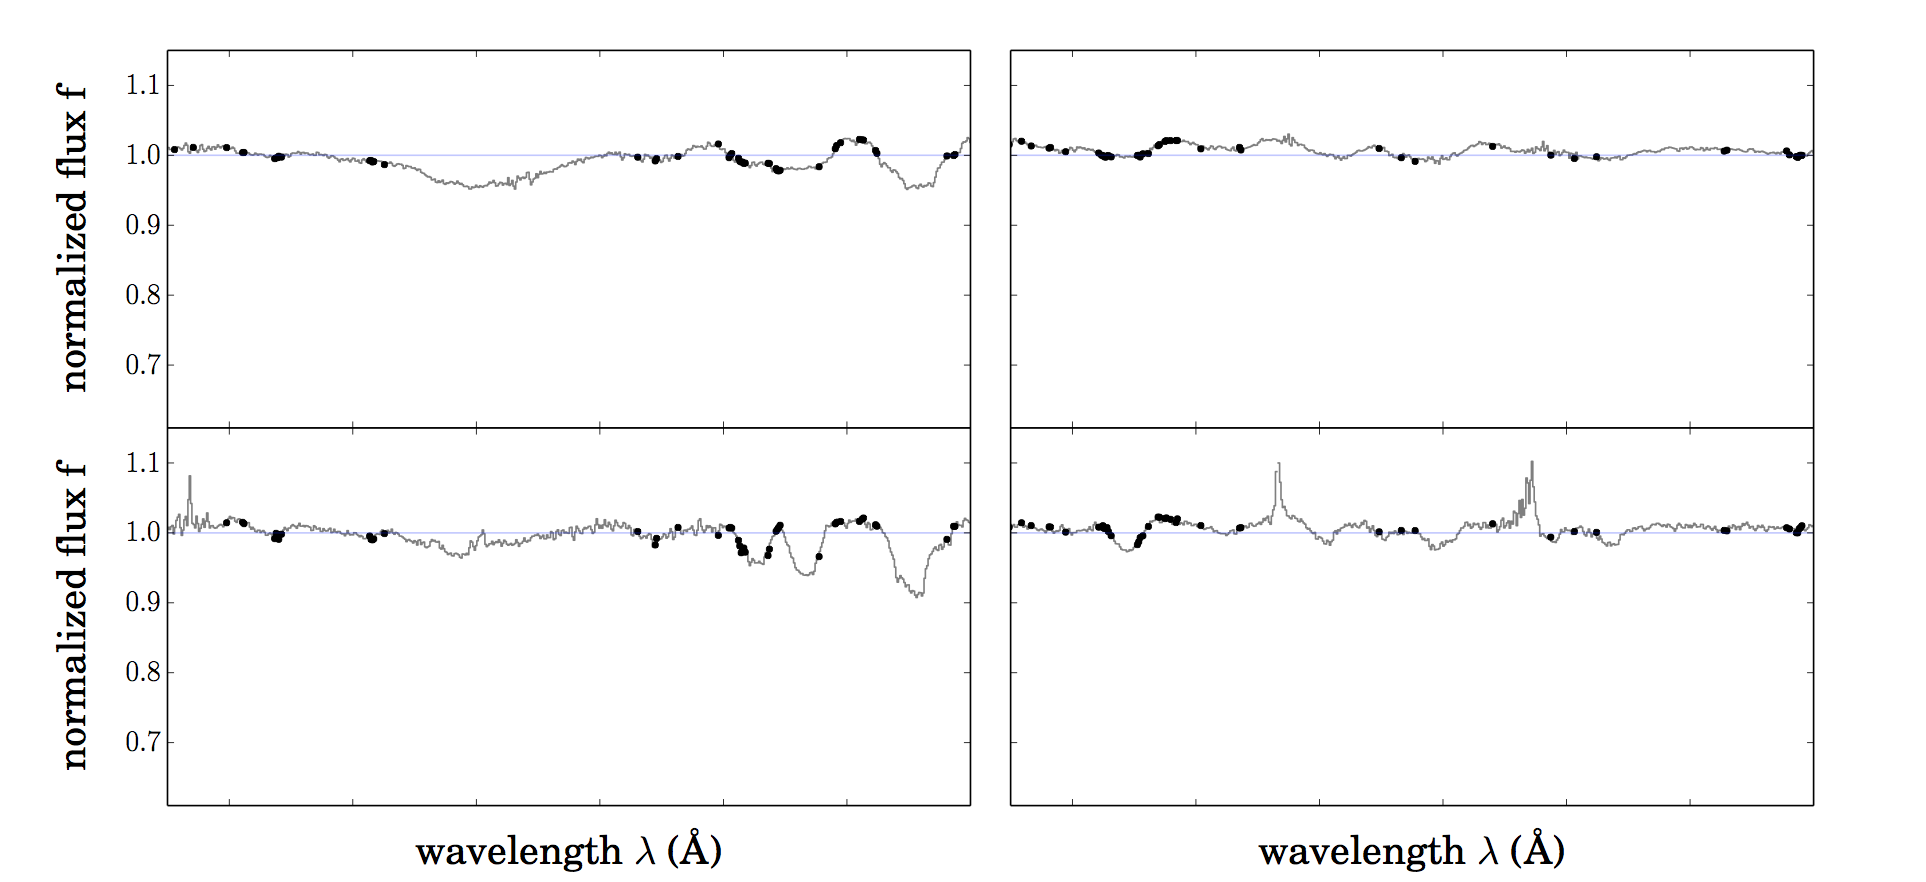
\includegraphics[width=\hsize]{./plots/2dwarfs.png}
  \caption{Examples of hot rotating dwarfs in the \apogee\ DR10 data across regions A and B, comparable to \figurename~\ref{fig:coeffs}. These types of stars are \textit{not} included in our set of reference objects. Therefore, the label transfer by \tc\ leads to grossly unphysical label estimates.}
\label{fig:dwarfs}
\end{figure}


The dwarf spectra in our reference set only come from the Pleiades cluster, at a single metallicity. 
This restricted sample limits our ability to determine the stellar parameters for dwarf stars. 
Given these training data, our model \textit{can} differentiate dwarfs from giants, as long as their spectra are comparable to that of the Pleiades. 
However, none of the dwarfs in our training set are hot rotating objects with broad line features. 
Three examples of stars with broad line features that are in the test data but not included in our training dataset are shown in \figurename~\ref{fig:dwarfs}.

It is possible to differentiate these stars with \tc\ because they are output in non-physical space in \teff-\logg, and present as a group of very metal poor, \feh\ $\sim$ --2.0, low \logg\ stars $\sim$ 0, with cool temperatures $\sim$ 4000 K. The metal poor solution determined by \tc\ reflects the dearth of lines in the spectra for these hot stars, given the training model. This group of stars is flagged in \aspcap\ with a \rotwarn\ flag set. We therefore are able to exclude these stars from our analysis using this condition. 
 



 \subsection{Performance at modest SNR}
 \label{sec:lowSNR}


By identifying `true' continuum pixels we have been able to implement a simple continuum normalisation that is robust across low and high SNR, which is valid across the parameter range of our training set. To examine how \tc\ performs at lower SNR, we have taken individual visits from the \apstar\ fits files, when there are $\ge$ 4 visits, and run \tc\ on a single visit spectra, when consistently continuum normalized (\sectionname~\ref{sec:ApogeeContinuum}) . Note, that we have not simply added noise to the combined DR10 spectra for our low SNR tests, which would bypass the question of how consistently the continuum can be defined at different SNR levels. Instead, we have treated single-visit spectra as (formally) independent survey objects. \figurename~\ref{fig:lowsnr} shows a comparison of a sample star for a single visit and combined visits ($>$ 4 total visits). \figurename~\ref{fig:SNR} presents the results of \tc\ compared to \apogee\ for these stars, showing \textit{only} the \apogee\ stars with errors of $<$ 150 K in \teff\ and $<$ 0.25 dex in \logg, across four SNR intervals, from 20 $<$ SNR $<$ 30 to 100 $<$ SNR $<$ 200.

These \figurenames\ illustrate that our approach to continuum normalization works well for both of these SNR regimes and is SNR independent, which is not true for a weighted-quantile normalisation. At the highest SNR (and \apogee\ estimates a upper noise floor of 200 although stars do measure above this), the rms difference between \tc\ and \aspcap\ is comparable to the \aspcap\ measurement errors, at 73K in \teff\, 0.18 dex in \logg\ and 0.11 dex in \feh. At a SNR of 30-50, the rms error increases to 100 K, 0.2 dex and 0.10 dex in \teff, \logg\ and \feh\, respectively. At an SNR of 20-30 the rms error is significantly higher and here the internal errors of \tc\ become comparable to typical minimisation methods and at SNR $<$ 20 exceed them. With this method we can return stellar parameters of \teff, \logg, \feh\ to as good a precisions as minimisation techniques ( \teff\ $<$ 100K, \logg\ $<$ 0.2 dex, \feh\ $< $0.1 dex) with an SNR of $\ge$ 25. 
 
%run -i makecontin_data1_revc.py
 \begin{figure}[!h]
  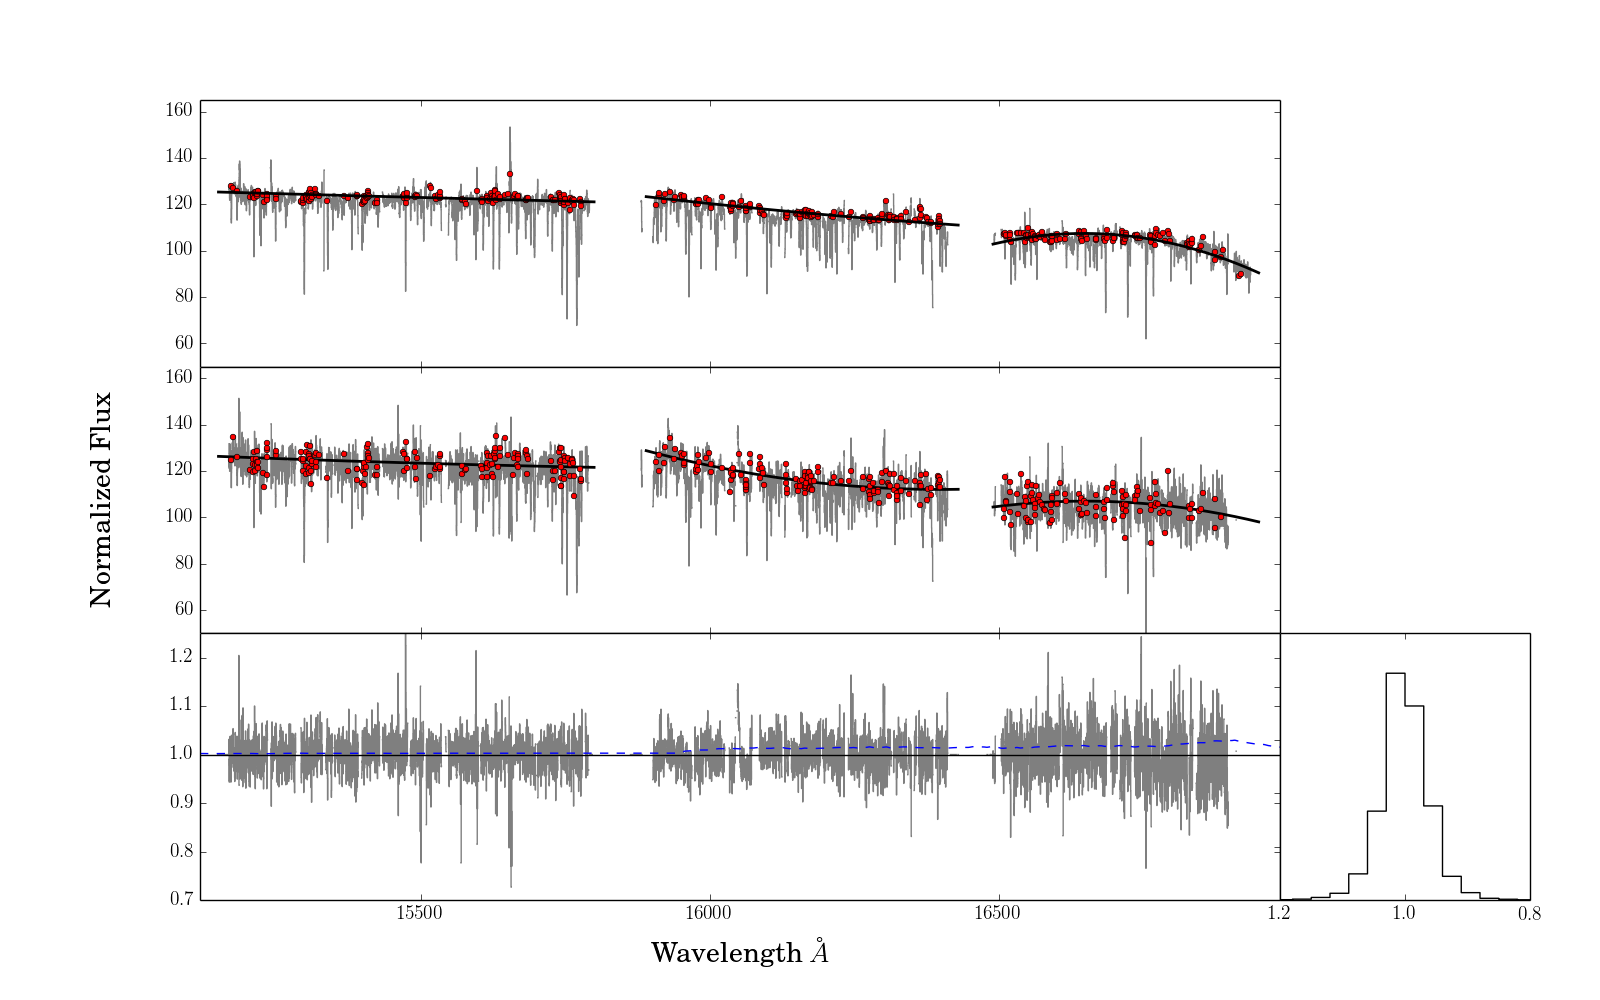
\includegraphics[width=\hsize]{./plots/SNR_continuum5.png}
  \caption{Comparison of the continuum normalisation of the same star at high and modest SNR. The \apogee\ \apstar\ combined visit spectra is shown in the top panel (SNR = 120) and the \apstar\ spectra for the 4th visit (SNR = 25) is shown in the second panel. The bottom panel is the ratio of the continuum normalised spectra of the high and medium signal to noise spectra and the blue dashed line is a running mean of this ratio, showing a small bias. The histogram of the ratio is given in at the right of the bottom panel.}
\label{fig:lowsnr}
\end{figure}

%makeplot_fits_SNRtest.py in /play but changed to makeplot_fits_SNRtest_bw.py
 \begin{figure}[!h]
 \centering
 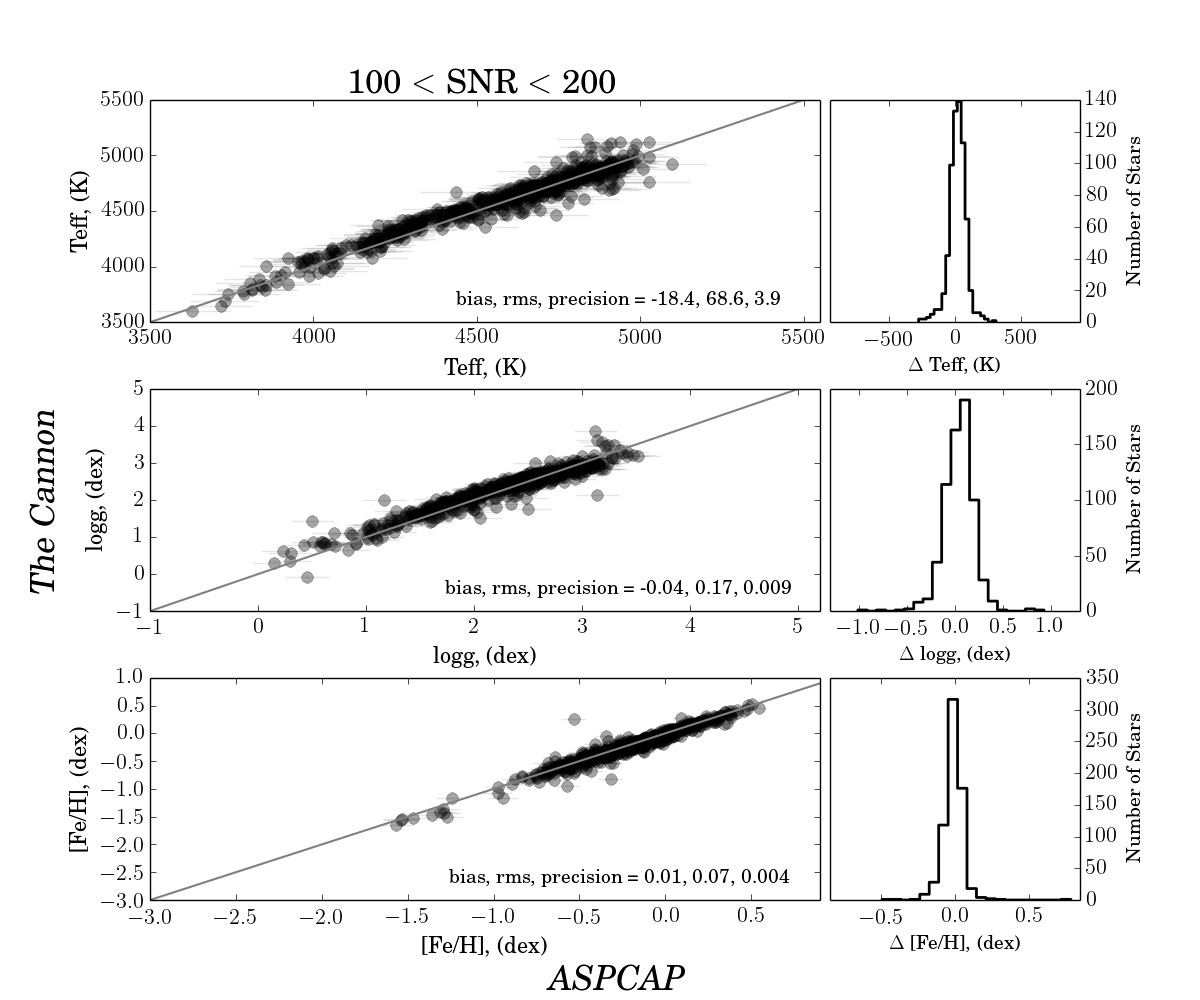
\includegraphics[scale=0.25]{./plots/SNR100to200.png}
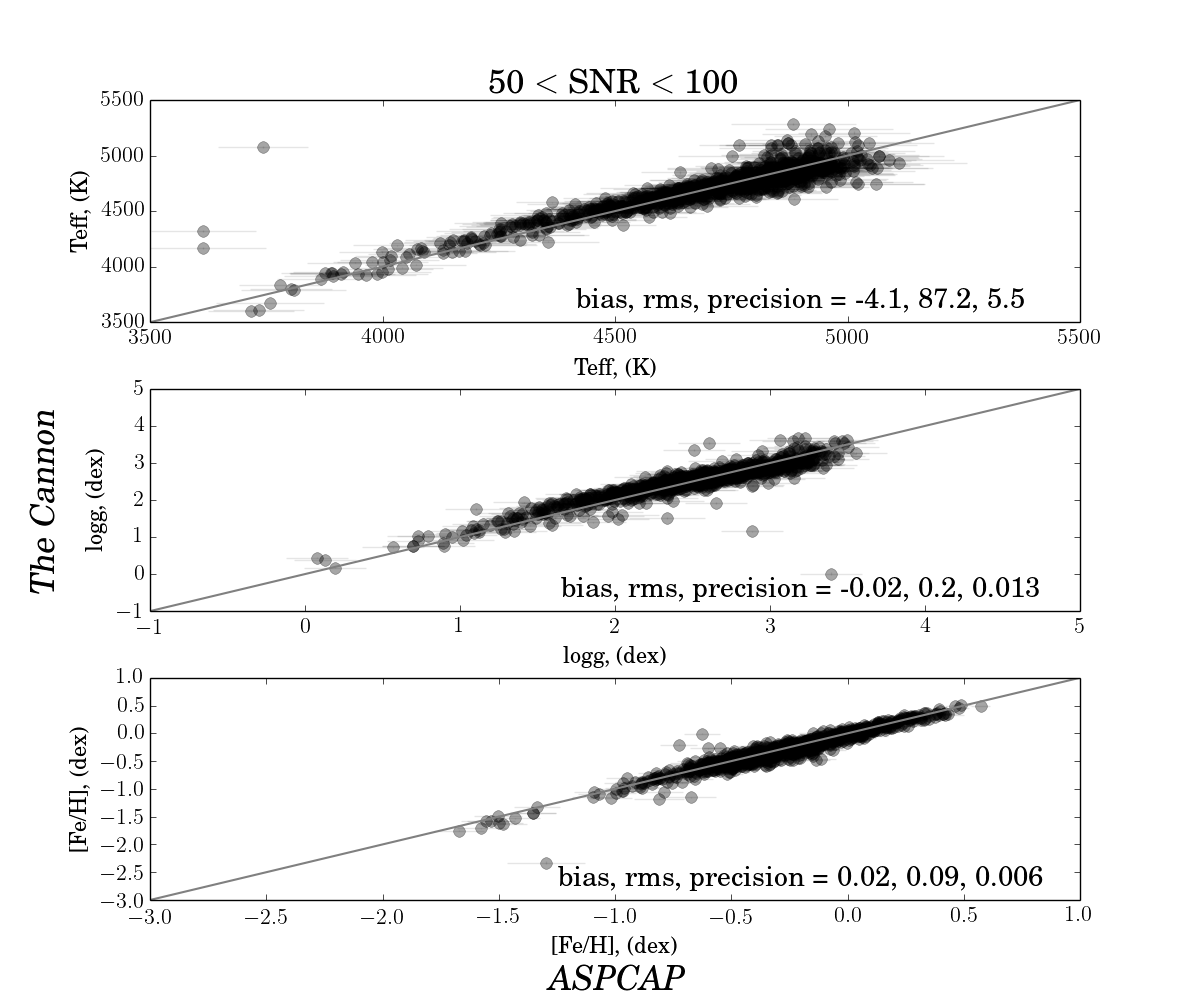
\includegraphics[scale=0.25]{./plots/SNR50to100.png}\\
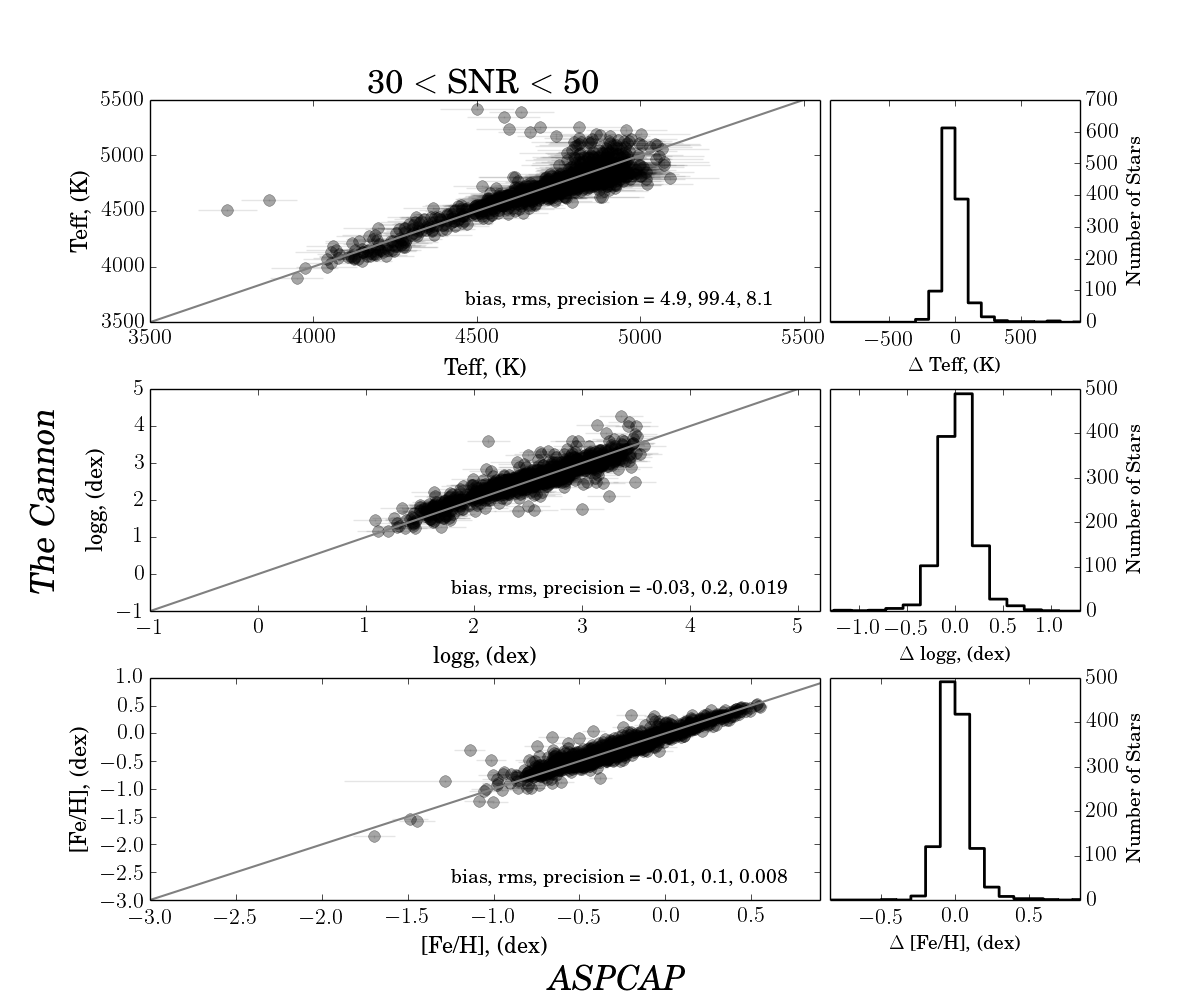
\includegraphics[scale=0.25]{./plots/SNR30to50.png}
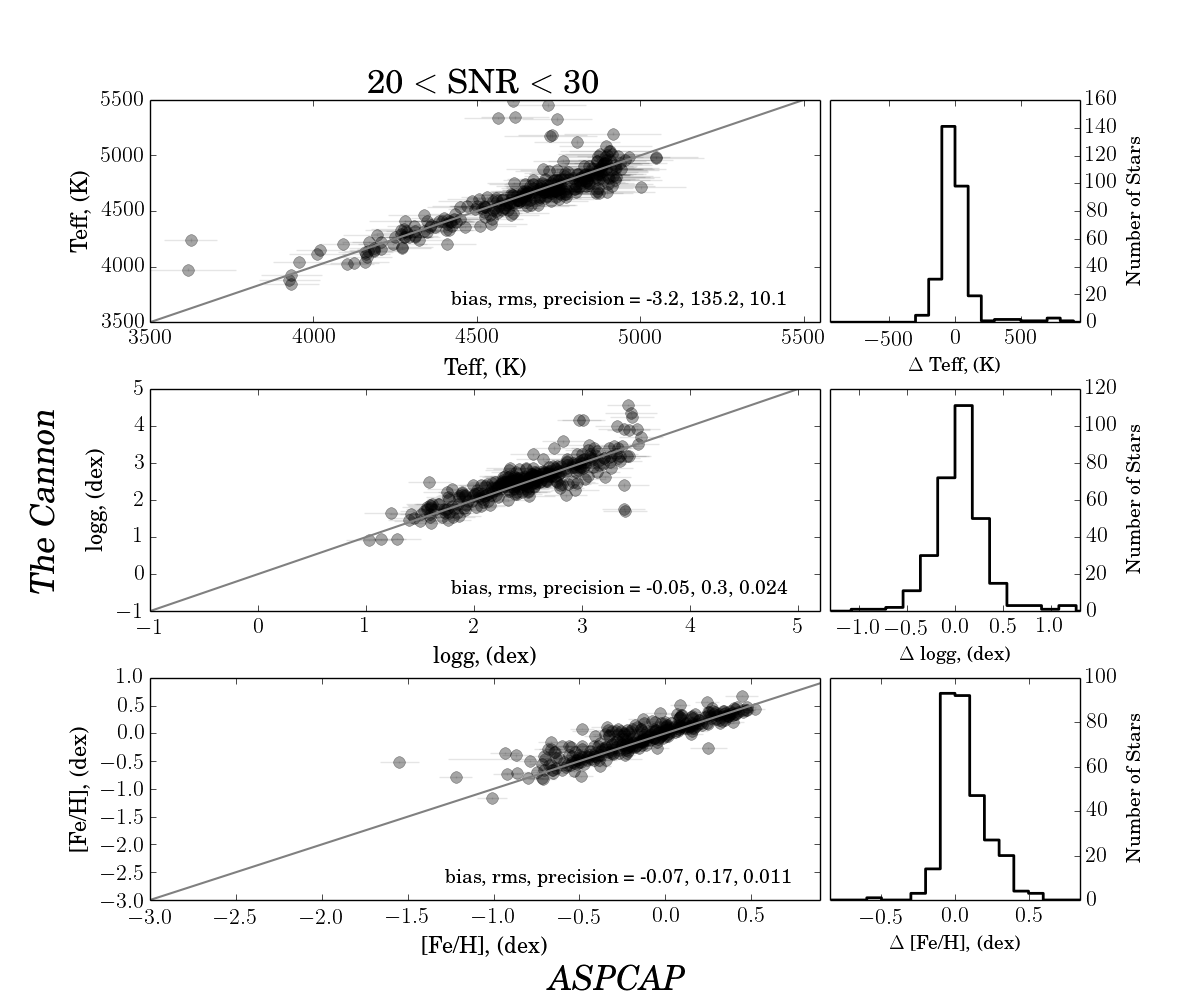
\includegraphics[scale=0.25]{./plots/SNR20to30.png}
    \caption{Illustration of \tc's ability to estimate labels for spectra of modest signal to noise. Shown is the comparison of \tc\ labels derived for some single visit spectra, compared to the \aspcap\ label values derived from the co-added high signal to noise spectra. The single vista spectra are grouped in four different regimes of signal to noise. There are 60 stars in the 300 $<$  SNR $<$ 30 bin, 1200 stars in the 30 $<$ SNR $<$ 50 bin, 1100 stars in the 50 $<$ SNR $<$ 100 bin and 670 stars in the 100 $<$  SNR $<$ 200 bin. Note that the rms difference between those two label estimates increases more slowly than expected from the signal to noise of the single visit spectra: label transfer with \tc\  therefore enables label estimates at modest signal-to-noise. Each SNR regime shows the corresponding histograms of \tc\ - \aspcap\ for each label, at right.}
\label{fig:SNR}
\end{figure}

\section{Discussion}

[DWH SAY: THIS PARAGRAPH IS WRONG - MKN SAYS: I changed it] We have demonstrated with \tc,  that using a data-driven model, labels can be transferred from training to test data, simply and efficiently. 
In using a data-driven model which spans the label range of the test data, we do not rely on explicit models in the wavelength region of analysis of the survey. 
We can therefore fully capitalise on large surveys and the information in the data itself, circumvent problems with simplified stellar models , uncertainties in linelists in poorly studied wavelength regions and understand where models are wrong.  

From our implementation of \tc\ on \apogee\ data, we were motivated to examine the calibration space of the labels given the unphysically narrow giant branch returned for DR10 data at low \logg. 
We found by adopting a very naive calibration that shifts the stars to the nearest position on the isochrone from the \aspcap\ value described in \sectionname~\ref{MKN REF}, the stars were returned in a \teff-\logg\ space, across metallicity, in line with expectations of the physical label-space of stars. 
This small \logg\ adjustment is naive, but works well, causing small offsets in the \logg\ scale at low temperatures and \logg\ values compared to the \apogee\ \logg\ input labels, which moves the stars onto the branches or the isochrones. 
This suggests that there is some problem with the input labels in the \logg\ dimension adjusted from Kepler results in DR10. 

For our first implementation of \tc\ presented here, it is trivial to run the 55,000 star sample (that is, the size of DR10 from \apogee) through \tc\ on a single laptop, as it takes $<$ 1/10$^{th}$ of a second (on a 2.6 GHz intel core i7) to determine three labels for each star, without any attempt at speed or method optimisation. 
We reproduce the \apogee\ labels, as provided for DR10 in Table 1, without adding any significant uncertainty because we use every pixel in the spectra and have a generative model. 
Our model is comprised of data which represents the probability space of the labels given the physical noise model,  where we let the noise model determine the weighting of the luminosity function, yet we can only do better. 

By returning coefficients, we have a tool which \textit{describes the flux in a quantitative way as a function of stellar labels}, thus removing degeneracies and improving the prospects for determining stellar parameters, by modelling covariance rather than attempting to minimise it. Regions that have dependencies on only one of the labels can also be easily identified. 

We have demonstrated that we can work at much lower SNR at least for the three primary stellar parameters with this approach. 
We expect to not gain the same advantage for individual elements with the SNR, but it may be possible to combine elements into subgroups (for example, alpha, light elements, neutron capture) of covariant spaces \citep[e.g.,][]{Ting2012}. In this way we exploit more pixels in the spectra and can operate at significantly lower signal to noise without being penalised in dimensionality of the returned parameter and abundance space. 
This suggests the possibility to dramatically either reduce the cost of survey, or multiply the number of stars observed by a factor of $\ge$ 2 for the same scientific gain. 

In using all of the pixels in the spectrum to obtain the
stellar labels, \tc\ is not dissimilar from the MATrix Inversion for
Spectral SythEsis (\matisse) procedure for derivation of stellar
parameters \citep{RB2006}.
That is, \matisse\ does well at low signal-to-noise for the same
reason as \tc:  They both use the full spectral range.
However, \matisse\ employs a large grid of synthetic spectra and
characterises a set of basis vectors which project onto each observed
spectrum to determine stellar labels by calculating an optimal
combined synthetic spectrum describing the stellar flux.
Conversely, we use a data-driven model and do not project onto any
subspace or combined theoretical spectrum.

 \tc\ is readily expandable to a more general model, a larger training dataset and many more labels which include errors and/or partial characterisation of labels. Furthermore we do not need to use all of the pixels in the spectra for our model and \tc\ can be generalised to use a linelist to select for particular regions or features.
 As it is, our second-order model is hard-coded and extremely restrictive. 
 We currently believe our input labels fully, given they are input without uncertainties, and assume no prior information. 
 We therefore do not take advantage of any physical knowledge that is defined about the phase space the labels can reside in.  
 Furthermore, we currently treat every pixel as independent which is incorrect and therefore builds a physically incomplete model.  As we lack dwarfs, we can not return parameters in this space to the same precision as giants (\logg\ $\le$ 3.5).  
 We also are missing any dwarfs with rotation in our model and consequently these are returned in an unphysical \teff-\logg\ label-space in the label-transfer. 

 %We have barely scratched the surface with what is possible with this methodology given our restricted training dataset, model and labels. 
 %Our training dataset itself is clearly too small, comprising only 545 stars including a set of dwarfs at a single metallicity (+0.03 dex). 

 
Although we use \apogee\ as an example, \tc\ can be applied to
any stellar survey.
Details of how the spectra are continuum-normalized might have to be
customized for different surveys, which will have different
line-spread functions and different absorption-line densities, and
therefore different statistics.
In all other respects, however, \apogee\ could be replaced by any spectroscopic
survey that meets the following criteria:
It must contain a set of reference stars with known labels to serve as
a training set.
It must deliver a set of spectra represented on a common rest-frame
wavelength basis.
It must deliver noise variance estimates at every spectral pixel.



The basic implementation of \tc\ presented here considers only three
labels (\teff, \feh, and \logg).
There is nothing fundamental abous this choice; in principle
\tc\ could be extended to consider more labels, or a larger
label space.
For example, a next generation could include \alphafe\ or \xfe\
labels for elements X.
The only limitation---and it is a \emph{substantial} limitation---is
that as the label-space grows, the training set must grow to fill it;
\tc\ is only as good as its training set.
In general, the training set needs may scale as badly as exponentially
with the dimensionality of the label space, and (as noted above), we
are confident that we don't have enough training stars even now with
a three-dimensional label space.
For this reason, we don't imagine operating \tc\ in the full 30-ish
dimensional label space imagined for the final outputs of surveys like
\apogee\ and \galah; \tc\ is only for establishing the ``first-order'' labels of
greatest importance in setting spectral properties.


In the above, we used a quadratic form for the
relationship between the expected flux and the labels.
This is a choice and can be generalized.
Indeed, the polynomial family is probably not the best family of
functions to be exploring, since they extrapolate badly (edge effects)
and require explicit, qualitative choices about order and cross-terms.
It is probably better to move to a non-parametric form for the functions,
such as Gaussian Processes or similar.
In this case, model complexity would be controlled by continuous
parameters and the functional form could become very complex where the
training data warrant it.
This would be a natural extension of what has been implemented here.

[DWH: SOMETHING ABOUT SPECTRAL REPRESENTATION]
%
%Despite all of this, we have shown using the \apogee\ data that even the simplest model with naive assumptions and an incomplete physical description, works. 
%This method is directly transferrable as is, to all other surveys and we expect we would be similarly successful applying this to e.g. \textit{GALAH}, \gaiaeso and 4MOST. 
%The success of \tc\ argues for defined stellar standards to effectively transfer labels of benchmark stars, studied at high resolution, to stars in surveys across any wavelength region. 
%This would enable all stellar surveys to be unified. 
 
 It is also possible and likely desirable in some cases to implement exactly the same procedure we describe using a synthetic grid instead of data, to train the model. 
 This will remove many of these limitations in the model that are derived from the label-space of the training data labels. However, this also eliminates many of the advantages in a full characterisation of the noise in the data and the true behaviour of labels with flux.
 
Given common benchmark stars observed between different surveys, these surveys can be unified on to a common scale with \tc. This approach can therefore optimally utilise the data that will be in hand in the coming years. 
 
 %,  we argue for adopting a wider set of benchmark stars from data in surveys, given labels determined at high resolution, in order to mitigate the issues with limited training datasets. 
 
%There are a number of immediate new opportunities with this approach. 
%The primary and obvious opportunity is to unify all stellar parameter systems and a key necessity of this is that all common benchmark stars be observed in all surveys. 
%The data-driven model approach enables an analysis and characterisation of how and where stellar templates diverge from data, but the ultimate consequence of this methodology is that by using the coefficients of the labels returned in this method for example in our quadratic implementation, we can directly identify and learn \textit{where} the information in a stellar spectrum resides. 
%This can be used to make quantitative assessments of the flux dependence on the labels, at the detail of the individual line profiles and, for example, determine continuum pixels as we have done to obtain a robust continuum normalisation across SNR. 
%The information in the spectra  is a direct output from the model, which is immensely more informative than the reverse assumption of assessing regions of interest as informed by linelists.  
%\tc\ is therefore extremely relevant for chemical tagging and we take an approach of a data-driven differential analysis of spectra, by characterising the behaviour of flux and labels, as a way to fingerprint stars with a common formation history.

%A direct first additional upgrade for \tc\ aligned with directing this method toward chemical tagging, which large surveys like \galah\ and \apogee\ have been constructed around,  is  to add more labels.
% An obvious initial choice is $\alpha$-enhancement and a subset of key individual abundances \xfe.
% It is even possible to test what, if any, information in the spectra are correlated with an age label. 
% If such information is present in the spectra across a large set of stars in a survey, this method \textit{will} determine exactly which pixels are responsible for carrying this information. In addition, we will gain significantly by moving to a more flexible model like a Gaussian process and allowing our model to be informed by priors in these new directions for this work. 

[MKN - removed/commented out some of the repetition DWH SAY:  THE DISCUSSION (above) IS A BIT REPETITIVE; WE CAN PROBABLY COMBINE AND SHORTEN PARAGRAPHS ABOUT GENERALIZATIONS.]

\textbf{DWH can you expand on generative models: data-driven model that represents the noise -  very successful as it respects the noise model. generative - synth, L.F. - permits discovery, interpretation.}


\section*{ Acknowledgements}

We would like to thank Daniel Foreman-Mackey (NYU), 
Morgan Fouesneau, Jon Holtzman,  Keivan Stassun and Jennifer Johnson
for valuable discussions.
DWH was partially supported by
the NSF (grant IIS-1124794), NASA (grant NNX08AJ48G), and the
Moore--Sloan Data Science Environment at NYU.
The research has received funding from the European Research Council under the European
Union's Seventh Framework Programme (FP 7) ERC Grant Agreement n.
[321035].

Funding for SDSS-III has been provided by the Alfred P. Sloan Foundation, the Participating Institutions, 
the National Science Foundation, and the U.S. Department of Energy Office of Science. The SDSS-III web site is $http://www.sdss3.org/.$\\

Funding for SDSS-III has been provided by the Alfred P. Sloan Foundation, the Participating Institutions, the National Science Foundation, and the U.S. Department of Energy Office of Science. The SDSS-III web site is $http://www.sdss3.org/.$\\

SDSS-III is managed by the Astrophysical Research Consortium for the Participating Institutions of the SDSS-III Collaboration
 including the University of Arizona, the Brazilian Participation Group, Brookhaven National Laboratory, Carnegie Mellon University, 
 University of Florida, the French Participation Group, the German Participation Group, Harvard University, the Instituto de Astrofisica 
 de Canarias, the Michigan State/Notre Dame/JINA Participation Group, Johns Hopkins University, Lawrence Berkeley National Laboratory, 
 Max Planck Institute for Astrophysics, Max Planck Institute for Extraterrestrial Physics, New Mexico State University, New York University, 
 Ohio State University, Pennsylvania State University, University of Portsmouth, Princeton University, the Spanish Participation Group, 
 University of Tokyo, University of Utah, Vanderbilt University, University of Virginia, University of Washington, and Yale University


\bibliography{tc3.bib}


\end{document}
